\documentclass{article}
% NeurIPS 2026 Evaluations \& Datasets (E\&D) Track submission.
% Anonymous double-blind is default. For arXiv preprint use: \usepackage[eandd, preprint]{neurips_2026}
% For optional single-blind (dataset-centric submissions): \usepackage[eandd, nonanonymous]{neurips_2026}
\usepackage[eandd]{neurips_2026}
\usepackage[utf8]{inputenc}
\usepackage[T1]{fontenc}
\usepackage{hyperref}
\usepackage{url}
\usepackage{booktabs}
\usepackage{array}
\usepackage{enumitem}
\usepackage{amsfonts}
\usepackage{amsmath}
\usepackage{amssymb}
\usepackage{nicefrac}
\usepackage{microtype}
\microtypesetup{expansion=false}
\usepackage{graphicx}
\usepackage{subcaption}
\usepackage{xcolor}
\usepackage{multirow}

\title{TabMI-Bench: Evaluating Mechanistic Interpretability Methods Across Tabular Foundation Model Architectures}

\author{
  Anonymous Author(s)
}

\begin{document}

\maketitle

\begin{abstract}
Mechanistic interpretability (MI) has matured rapidly for large language models, yet no reusable evaluation framework exists for the growing ecosystem of Tabular Foundation Models (TFMs). We introduce \textbf{TabMI-Bench}, a \emph{protocol benchmark} that documents, for the first time, \emph{which} MI techniques remain informative on \emph{which} TFM architectures. Its three concrete deliverables are (i)~a uniform hook-based activation-extraction layer for 5 TFMs spanning 3 architectural families, (ii)~an \emph{evidence-coded MI applicability matrix} over 8 techniques, and (iii)~a 4-step evaluation protocol (synthetic probe $\to$ causal validation $\to$ negative controls $\to$ real-world transfer) with reference baselines.

A primary diagnostic finding is that whole-layer clean activation patching is \emph{uninformative} in the tested ICL-style TFMs because shared weights and fixed inputs cause any clean replacement to cascade deterministically through downstream layers; corruption-based (noising) tracing is the informative alternative. As calibration, three descriptive reference computation profiles emerge in the tested model set --- \textit{staged} (TabPFN), \textit{distributed} (TabICL, TabDPT), and \textit{preprocessing-dominant} (iLTM) --- 5-seed replicated on the three core models across 4 function types, with in-family (TabDPT) and out-of-family (NAM) holdouts. Supporting analyses cover noising-based causal tracing on 11 real-world datasets (3 seeds) and 5-seed steering on 4 regression datasets where direction is consistently detectable ($|r|{>}0.70$ TabPFN; $>0.94$ TabICL) but per-dataset effect-size magnitude is dataset-dependent, plus SAE scaling to $256\times$ expansion. Hook implementations, synthetic generators, frozen artifacts, a benchmark card, and Croissant metadata will be released.
\end{abstract}

\section{Introduction}

Tabular Foundation Models (TFMs) represent a rapidly evolving class of pre-trained models that can perform prediction tasks on arbitrary tabular datasets without task-specific training. Models such as TabPFN~\cite{hollmann2025tabpfn}, TabICL~\cite{qu2025tabicl}, and iLTM~\cite{ye2025iltm} achieve competitive or superior performance relative to XGBoost and other gradient-boosted decision trees (GBDTs) on small-to-medium datasets ($n < 10{,}000$), often with zero-shot or few-shot inference.

As TFMs are deployed in high-stakes domains --- credit scoring, medical diagnosis, insurance pricing --- understanding \textit{how} they arrive at predictions becomes critical. Unlike large language models (LLMs), where mechanistic interpretability (MI) has rapidly progressed through techniques such as probing~\cite{alain2016understanding}, logit lens~\cite{nostalgebraist2020logitlens}, activation patching~\cite{heimersheim2024activation}, and sparse autoencoders (SAEs)~\cite{bricken2023towards}, tabular foundation models remain largely uninterpreted.

Prior TFM MI work is largely single-model and correlational. Gupta et al.~\cite{gupta2026tabpfn} applied linear probing and logit lens to TabPFN v2, finding that TabPFN encodes regression coefficients in intermediate layers and forms predictions around layer 5--8. Balef et al.~\cite{balef2025layers} report complementary layer-wise observations. Both studies focus on a single architecture with correlational tooling. TabMI-Bench builds on these as reference baselines within a broader, causally-validated, cross-architecture benchmark.

\textbf{Contributions.} TabMI-Bench makes four scoped contributions, ordered by how directly they create reusable community infrastructure:

\begin{enumerate}
\item \textbf{Reusable MI infrastructure and evaluation protocol.} Hook-based activation extraction for 5 TFMs (with known model-specific limitations documented in the release), controlled synthetic probes (4 function types), a 4-step evaluation protocol for new methods/models, and a benchmark output schema that reports profile metrics, causal validation, controls, and transfer checks.
  \item \textbf{Evidence-coded MI applicability matrix with a concrete diagnostic finding.} The matrix records, for 8 MI techniques across 4 tested architectures, which methods yield architecture-consistent signal (Supported), partial signal (Limited), or were not tested (Not established), with explicit seed-count superscripts. Its primary diagnostic finding is that \emph{whole-layer clean activation patching is uninformative on the tested ICL-style TFMs} due to deterministic cascading (replacing layer-$L$ activations with their clean counterparts cascades unchanged through all downstream layers), and corruption-based tracing is the informative alternative.
  \item \textbf{Three descriptive reference computation profiles for calibration.} Staged (TabPFN), distributed (TabICL, TabDPT), and preprocessing-dominant (iLTM), 5-seed replicated on the three core models across 4 function types, with profile-level variance metrics, negative controls, function-invariance checks, and two holdouts (in-family TabDPT; out-of-family NAM).
  \item \textbf{Supporting analyses with explicit evidence tiers.} Real-world steering transfer (5-seed, $|r| > 0.70$ TabPFN / $> 0.94$ TabICL on 4 datasets), architecture-dependent SAE scaling behavior (up to $256\times$ expansion), and $100\times$ scale validation (3-seed probing, profiles preserved).
\end{enumerate}

\section{Background and Related Work}

We study five TFMs spanning three architectural families: dual-axis transformers (TabPFN v2~\cite{hollmann2025tabpfn} and v2.5~\cite{priorlabs2025tabpfn25}), column-to-row transformers (TabICL v2~\cite{qu2025tabicl} and TabDPT~\cite{somboonvorakul2024tabdpt}), and a tree+MLP hybrid (iLTM~\cite{ye2025iltm}). \textit{Selection criteria}: we include five representative open TFMs that (a)~perform in-context or zero-shot tabular prediction, (b)~had open-source checkpoints at the time of our experiment freeze (January 2026), and (c)~expose internal layer activations for hook-based extraction. This excludes closed-source models and non-ICL tabular methods (XGBoost, LightGBM). The main statistically validated comparison uses three core models (TabPFN, TabICL, iLTM). Including iLTM --- a non-Transformer model with only 3 MLP layers after RF+PCA preprocessing --- is essential: without it, the study could not test whether the observed profiles are tied to transformer internals or persist in a qualitatively different tabular architecture. TabDPT and TabPFN v2.5 serve as supporting analyses. Models published after our freeze (e.g., KernelICL~\cite{miftachov2026kernelicl}) can be added via the hook interface ($\sim$150 lines; see Appendix~\ref{app:architecture}).

We apply standard MI tools from language-model analysis --- probing, logit lens, activation interventions~\cite{turner2023activation}, steering, sparse autoencoders, CKA, and attention analysis --- but focus on which of these remain informative in the tabular in-context setting. Recent concurrent work on TFM fairness~\cite{kenfack2025fairness} and feature interaction learning~\cite{karabulut2026association} complements our focus on internal computation. Prior tabular MI work is largely correlational and model-specific~\cite{gupta2026tabpfn,balef2025layers}. In the language-model domain, the Mechanistic Interpretability Benchmark (MIB)~\cite{mueller2025mib} evaluates circuit localization and causal variable identification across LLMs. TabMI-Bench serves an analogous role for the tabular domain but differs in three design respects driven by TFM-specific constraints: (i)~TFM architectural heterogeneity (dual-axis vs.\ column-row vs.\ tree+MLP) directly changes \textit{which} MI methods are applicable, so method-level applicability mapping is a first-class output; (ii)~TFMs lack the token-level semantics that enable circuit-level objectives in LLMs, so our primary unit is the layer-level computation profile rather than individual circuits; (iii)~the TFM ecosystem is smaller and younger, so we provide a protocol scaffold with reference baselines rather than a scored leaderboard. Our contribution is reusable evaluation infrastructure with causal validation, not a domain adaptation of MIB.

\textbf{Relation to tabular benchmarks.} Existing tabular benchmarks (TabZilla~\cite{mcelfresh2024tabzilla}, TabReD~\cite{rubachev2024tabred}, OpenML-CC18) evaluate \textit{predictive performance} --- accuracy, calibration, runtime --- across models and datasets. They do not evaluate internal computation. TabMI-Bench targets a complementary axis: \textit{which MI methods are informative for which architectures, and where does computation happen inside these models?} This requires infrastructure absent from performance benchmarks: hook-based activation extraction, synthetic probes with known intermediary variables, and causal intervention protocols. Extending an existing performance benchmark with MI evaluation would be insufficient because MI evaluation requires controlled ground-truth targets (our synthetic probes) and model-internal access (our hook interface) that performance benchmarks do not provide.

Cross-architecture representation comparisons in vision and across modalities motivate our setup~\cite{zhou2022understanding,sirikova2026architecture,hosseini2025universality}, while recent work on causal tracing, automated circuit discovery, cross-model SAEs, and steering informs our analysis choices~\cite{meng2022locating,conmy2023acdc,marks2024sparse,mueller2024quest,jiralerspong2026crosscoders,kendiukhov2026causal,staniszewski2026tada,yang2026steplevel}. Additional architectural details and technique inventories are deferred to Appendix~\ref{app:architecture}.

\section{Methodology}

\textbf{Controlled synthetic probes.} We use four synthetic task families as controlled interpretability probes: (1)~coefficient probing ($z = \alpha x + \beta y$), (2)~bilinear intermediary probing ($z = a \cdot b + c$), (3)~sinusoidal intermediary probing ($z = \sin(a \cdot b) + c$), and (4)~polynomial intermediary probing ($z = a^2 + b \cdot c$). These probe functions are designed around three principles: \textit{controllability} --- each has a known intermediary variable that can be targeted by linear probes; \textit{interpretability} --- causal interventions (noising, steering) produce predictable effects; and \textit{diversity} --- the four functions span linear, bilinear, trigonometric, and polynomial relationships, testing whether computation profiles are invariant to the target function type. Core experiments use $N_\text{train}=100$, $N_\text{test}=50$ and the canonical 5 random seeds $\{42,123,456,789,1024\}$. We recommend $\geq 5$ seeds as the minimum for benchmark comparisons. Supporting experiments that use 3 seeds are marked as \textit{preliminary}. The $N{=}10$K scaling check for intermediary probing uses 3 seeds; its steering sub-check remains single-seed due to computational cost.

\textbf{Interpretability methods.} We extract layer activations from all model families and evaluate them with linear probing, logit lens (TabPFN only), noising-based causal tracing, steering vectors, sparse autoencoders, CKA, and attention analysis. Our primary causal tool is corruption-based tracing: standard clean activation patching is uninformative in these ICL-style TFMs because clean activations deterministically propagate through downstream layers (\S\ref{sec:controls}).

\textbf{Statistical plan.} We pre-specify two primary endpoints and their tests: (1)~\textit{profile difference}: layer-wise intermediary $R^2$ variance (not peak $R^2$ alone) compared between TabPFN and TabICL via exact permutation test; (2)~\textit{causal locus difference}: noising sensitivity profiles compared via exact permutation test. Secondary endpoints (steering, SAE, v2.5, real-world transfer) use the same test family but are interpreted as supporting evidence. Multiple-testing correction uses Bonferroni over the 5 tests in Table~\ref{tab:stats}, with BH-FDR reported for context. We summarize computation profiles using \textit{profile-level metrics} rather than peak values alone: layer-wise $R^2$ variance ($\sigma^2_\text{profile}$) captures how concentrated vs.\ distributed computation is, and the minimum per-layer $R^2$ captures dip depth (low for staged U-shape, near-peak for flat distributed profiles). The post-hoc taxonomy (staged/distributed/preprocessing-dominant) is a descriptive summary of these metrics, not a pre-registered classification. \textit{Unit of analysis}: each seed produces one profile summary statistic (e.g., one $\sigma^2_\text{profile}$ value) for the primary comparison. Permutation tests are performed over these seed-level summaries to avoid pseudo-replication across layers. With 5 seeds per group, the minimum two-sided $p$ is $1/\binom{10}{5} \approx 0.004$. We pre-specify family-wise $\alpha = 0.05$, giving Bonferroni threshold $\alpha_{\text{Bonf}} = 0.05/5 = 0.01$ over the 5 tests; raw $p$ values are reported alongside effect-size separation as joint evidence.

\textbf{Real-world transfer.} We validate two MI techniques on real-world data: (1)~noising-based causal tracing on 11 OpenML datasets, testing transfer of architecture-linked layer-sensitivity signatures; and (2)~steering vectors on 4 regression datasets (California Housing, Diabetes, Wine Quality, Bike Sharing), using median-split contrastive directions to test whether steering produces monotonic prediction shifts outside the synthetic regime. One additional dataset (Concrete) was excluded due to an OpenML cache failure. Full model specifications, hook details, and extended protocol information are provided in Appendix~\ref{app:architecture}.

\textbf{Evidence tiers.} Table~\ref{tab:evidence-tiers} makes the strength of each claim explicit: Core claims are backed by 5-seed replication with negative controls passed; Supporting claims have 3--5 seeds but are framed as secondary; Preliminary claims are single-seed or quick-run.

\begin{table}[h]
\centering
\caption{Evidence tiers for the main claims. Each tier links the claim to the seed count, artifact, and status of negative controls.}
\label{tab:evidence-tiers}
\scriptsize
\setlength{\tabcolsep}{4pt}
\begin{tabular}{@{}p{5.6cm} l c >{\raggedright\arraybackslash}p{5.6cm}@{}}
\toprule
Claim & Tier & Seeds & Source artifact \\
\midrule
3-profile taxonomy on TabPFN/TabICL/iLTM & Core & 5 & \texttt{rd5\_fullscale/aggregated/*.json} \\
Function invariance across 4 functions & Core & 5 & \texttt{phase8a\_nonlinear\_probing/*.json} \\
Deterministic cascading (clean patching) & Core & 5 & \texttt{rd5\_fullscale/patching/*.json} \\
Noising-based causal profile difference & Core & 5 & \texttt{rd5\_fullscale/patching/*.json} \\
Synthetic steering effectiveness & Core & 10 & \texttt{rd6\_fullscale/robust\_steering/*.json} \\
Real-world causal transfer (11 datasets) & Supporting & 3 & \texttt{phase7/realworld\_causal/*.json} \\
Real-world steering (4 datasets) & Supporting & 5 & \texttt{phase8b/realworld\_steering\_multiseed/*} \\
SAE scaling (architecture-dependent) & Supporting & 5--10 & \texttt{phase7/sae\_scaling\_*.json} \\
NAM out-of-family holdout & Supporting & 5 & \texttt{phase9\_nam\_holdout/*.json} \\
$N{=}10$K scale validation (probing) & Supporting & 3 & \texttt{scale\_10k\_multiseed/*.json} \\
TabDPT in-family holdout & Supporting & 3 & \texttt{phase7/tabdpt\_probing/aggregated\_3seed.json} \\
TabPFN v2.5 comparison & Supporting & 3 & \texttt{rd6/tabpfn25\_fullscale/aggregated/*.json} \\
\bottomrule
\end{tabular}
\end{table}

\textbf{Scope.} TabMI-Bench evaluates \textit{where} computation happens (layer-level profiles) and \textit{which MI methods apply} to which architectures. It does not evaluate \textit{what} is computed at the circuit level (individual attention heads, MLP neurons) or provide feature-level attribution. Circuit-level analysis requires model-specific tools (e.g., ACDC~\cite{conmy2023acdc}) that are beyond the current benchmark's scope but are a natural extension.

\textbf{Benchmark output.} A TabMI-Bench evaluation produces a structured result consisting of five components:

\begin{table}[t]
\centering
\caption{TabMI-Bench structured output components for evaluating a new MI method or profiling a new TFM.}
\label{tab:benchmark-output}
\small
\begin{tabular}{@{}l l l l@{}}
\toprule
Component & Metric & Required? & Interpretation \\
\midrule
Synthetic profile & $\sigma^2_\text{profile}$, min/peak $R^2$ & Yes & staged vs.\ distributed \\
Causal validation & sensitivity profile agreement & Yes & causal relevance \\
Negative controls & null detection pass/fail & Yes & method sanity \\
Real-world transfer & signature transfer summary & Recommended & beyond synthetic \\
Applicability & qualitative support label & Yes & practical usability \\
\bottomrule
\end{tabular}
\end{table}

\noindent This output structure (Table~\ref{tab:benchmark-output}) applies both to evaluating a new MI technique (compare its synthetic profile and causal validation against the reference baselines in Table~\ref{tab:three-strategies}) and to profiling a new TFM (classify its $\sigma^2_\text{profile}$ and min $R^2$ relative to the staged/distributed/preprocessing-dominant reference ranges).

\textbf{Applicability labeling rule.} The applicability matrix (Appendix~\ref{app:mi-full}) assigns each method--model pair one of three labels: \textit{Supported} ($\checkmark$) --- the method yields architecture-consistent signal, passes negative controls, and produces reproducible results across the stated seeds; \textit{Limited} ($\triangle$) --- informative signal exists but only for a subset of models, layers, or tasks, or control coverage is incomplete; \textit{Not established} ($\times$) --- the method was not tested on this model, or evidence is insufficient. Crucially, $\times$ means ``not tested,'' not ``does not work.''

\textbf{Improvement criterion.} TabMI-Bench does not produce a single scalar score. A new MI method $M'$ is considered to \textit{improve over} an existing method $M$ if: (i)~$M'$ achieves stronger profile--reference agreement (higher $R^2$ or lower profile distance) on the synthetic suite; (ii)~$M'$'s identified layers are confirmed by the causal validation protocol; and (iii)~$M'$ passes the same negative controls. This is a structured comparison, not a ranking --- methods may improve on some components while being equivalent or weaker on others.

\textbf{Evaluation protocol for new methods.} TabMI-Bench is designed so that new MI techniques or new TFMs can be evaluated against the reference baselines. The recommended protocol is:
\begin{enumerate}[nosep,leftmargin=*]
\item \textit{Synthetic evaluation}: Run the new method on all 4 synthetic function types with $\geq 5$ seeds. Compare layer-wise profiles against Table~\ref{tab:three-strategies}.
\item \textit{Causal validation}: Verify that identified layers are causally relevant using the noising-based causal tracing protocol (\S\ref{sec:causal}).
\item \textit{Negative controls}: Confirm that the method yields null results on random-target probing and random-vector steering baselines (Appendix~\ref{app:controls}).
\item \textit{Real-world transfer}: Evaluate on the 11-dataset causal tracing suite and 4-dataset steering suite (Table~\ref{tab:realworld-steering}) to test generalization beyond synthetic tasks.
\end{enumerate}
For adding a new TFM, the researcher implements a hook class following the \texttt{HookedModel} interface (Appendix~\ref{app:architecture}), which requires $\sim$100--200 lines of code and exposes \texttt{forward\_with\_cache()}, \texttt{get\_layer\_activations()}, and \texttt{num\_layers}. The existing experiment scripts then run without modification. A worked example (\texttt{examples/add\_new\_model.py}) and a benchmark card (\texttt{BENCHMARK\_CARD.md}) are included in the release.

\section{Results}

\subsection{Three Computation Strategies}
\label{sec:strategies}

\textbf{Figure~\ref{fig:intermediary}} shows intermediary $R^2$ profiles across layers for all four models. Taken together, these profiles motivate a compact descriptive summary of three recurring computation strategies:

\textbf{Operational definitions.} We classify a model as \textit{staged} if its intermediary $R^2$ profile shows $>$0.15 absolute variation across layers and a \emph{non-monotone} shape (at least one internal layer below both its neighbors --- e.g., a U or V); as \textit{distributed} if $R^2 > 0.90$ at every layer with $<$0.08 absolute variation; and as \textit{preprocessing-dominant} if the peak occurs in the first half of layers \emph{and} $R^2$ drops by $>$0.15 from peak to final layer. Rules are applied in the order distributed $\to$ staged $\to$ preprocessing-dominant; the first match wins. These criteria are post-hoc descriptors of the observed profiles, not pre-registered hypotheses. The thresholds are robust: perturbing them by $\pm 50$\% (e.g., staged threshold from 0.10 to 0.23) does not change the classification of any of the 5 models, because the inter-architecture gaps are large (TabPFN absolute variation $\approx 0.52$ vs.\ TabICL absolute variation $< 0.01$).

\begin{table}[t]
\centering
\caption{Intermediary probing profiles, profile-level variance ($\sigma^2_\text{profile}$), minimum $R^2$ across layers, and inferred strategies. Profile variance captures how concentrated vs.\ distributed computation is across layers; the minimum $R^2$ captures dip depth (low for staged U-shape, high for distributed/flat). TabPFN/TabICL/iLTM values are computed from \texttt{rd5\_fullscale/aggregated/aggregated\_results.json}; TabDPT values are computed from \texttt{phase7/tabdpt\_probing/aggregated\_3seed.json}. Peak $R^2$ is mean$\pm$std across per-seed peaks; $\sigma^2_\text{profile}$ is computed on the mean profile across seeds.}
\label{tab:three-strategies}
\small
\begin{tabular}{@{}l l c c c l@{}}
\toprule
Model & Profile & Peak $R^2$ & $\sigma^2_\text{profile}$ & Min $R^2$ & Strategy \\
\midrule
\textbf{TabPFN} & U-shape (dip L2--3) & $0.984 \pm 0.003$ & $0.033$ & $0.461$ (L2) & \textbf{Staged} \\
\textbf{TabICL} & Flat high ($> 0.99$) & $0.998 \pm 0.001$ & $<10^{-4}$ & $0.990$ (L11) & \textbf{Distributed} \\
\textbf{TabDPT} & Flat high ($> 0.989$) & $0.997 \pm 0.001$ & $2{\times}10^{-6}$ & $0.992$ (L9) & \textbf{Distributed} \\
\textbf{iLTM} & Mid-then-drop at L2 & $0.980 \pm 0.005$ & $0.018$ & $0.715$ (L2) & \textbf{Preproc.-dom.} \\
\bottomrule
\end{tabular}
\end{table}

\begin{figure}[t]
  \centering
  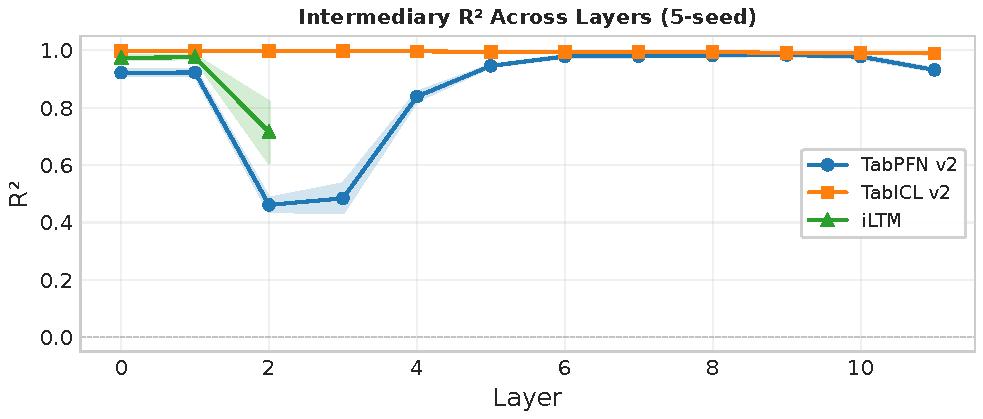
\includegraphics[width=0.68\textwidth]{figures/fig1_intermediary_r2.pdf}
  \caption{Intermediary probing $R^2$ across layers for TabPFN (12 layers, 5 seeds), TabICL (12 blocks, 5 seeds), TabDPT (16 layers, 3 seeds), and iLTM (3 layers, 5 seeds). Shaded bands show $\pm$1 std over seeds. TabPFN exhibits a characteristic U-shape (staged computation), TabICL and TabDPT maintain high $R^2$ uniformly (distributed), and iLTM peaks at L0 then decays (preprocessing-dominant).}
  \label{fig:intermediary}
\end{figure}

The profile-level variance ($\sigma^2_\text{profile}$) quantifies the difference: TabPFN has high variance ($0.033$), indicating concentrated computation, while TabICL is essentially flat ($\sigma^2 < 10^{-4}$). This difference is statistically significant using the pre-specified primary endpoint (exact permutation test on per-seed $\sigma^2_\text{profile}$: $p = 0.008$; Cohen's $d = 9.79$; 95\% CI for TabPFN peak $R^2$: $[0.981, 0.988]$, TabICL: $[0.997, 0.999]$). Given the small number of seeds, we treat the permutation result and the orders-of-magnitude separation in profile variance as stronger evidence than the magnitude of Cohen's $d$ alone.

\textbf{TabPFN (Staged):} Information is selectively processed in a stage-wise manner. Layers 0--1 perform initial encoding, layers 2--4 show a characteristic dip in intermediary recoverability, and layers 5--8 concentrate the core computation. This U-shaped profile is consistent with the findings of Gupta et al.~\cite{gupta2026tabpfn}.

\textbf{TabICL (Distributed):} Information is uniformly available across all 12 ICL blocks. The $R^2$ remains above 0.93 at every layer, with only a gradual decline. This is consistent with TabICL's column-then-row attention design supporting broad information availability rather than a narrow bottleneck layer.

\textbf{iLTM (Preprocessing-Dominant):} Peak information is at L1 ($R^2{=}0.976$) with L0 within $\pm0.002$, then decays at L2 to 0.715. The Random Forest + PCA preprocessing performs the heavy computational lifting; the 3-layer MLP refines rather than transforms.

\textbf{TabDPT (Distributed, 3-seed in-family holdout).} TabDPT maintains intermediary $R^2 > 0.989$ across all 16 layers on every seed, with peak $R^2 = 0.997 \pm 0.001$ at L3 and $\sigma^2_\text{profile} = 2\times10^{-6}$ ($n_\text{train}{=}50$, seeds $\{42, 123, 456\}$). The flat-high profile matches TabICL's qualitatively despite larger scale (16 layers / 768$d$ vs.\ 12 layers / 512$d$), providing 3-seed in-family evidence that the column$\to$row attention topology preserves the distributed pattern as model size grows. Causal validation (3 seeds) further confirms the distributed signature: noising-based sensitivity peaks at L0 on every seed (mean normalized sensitivity $1.00 \to 0.03$ from L0 to L15), matching TabICL's input-dominant pattern. The orders-of-magnitude separation from the staged threshold ($\sigma^2_\text{profile} = 2\times10^{-6}$ vs.\ TabPFN's $0.033$) renders the distributed classification unambiguous.

\textbf{CKA as a secondary check} (full heatmaps in Appendix~\ref{app:cka}). TabPFN's CKA matrix shows a clear 3-block structure (L0--1, L2--4, L5--11) with adjacent-layer CKA as low as 0.04 at block boundaries --- consistent with staged computation. TabICL is nearly uniform (adjacent CKA 0.73--0.99), iLTM shows a smooth 3-layer gradient (0.43--0.86). The three CKA patterns match the three probing-derived strategies.

\subsection{Function Invariance}

A natural concern is whether the computation profiles are artifacts of the simple bilinear task ($z = a \cdot b + c$). To test this, we repeat intermediary probing and causal tracing with three additional non-linear target functions: sinusoidal ($z = \sin(a \cdot b) + c$), polynomial ($z = a^2 + b \cdot c$), and mixed ($z = \sin(a \cdot b) + a \cdot b \cdot c$). Figure~\ref{fig:function-invariance} shows the full layer-wise $R^2$ profiles overlaid by function type.

\begin{figure}[t]
  \centering
  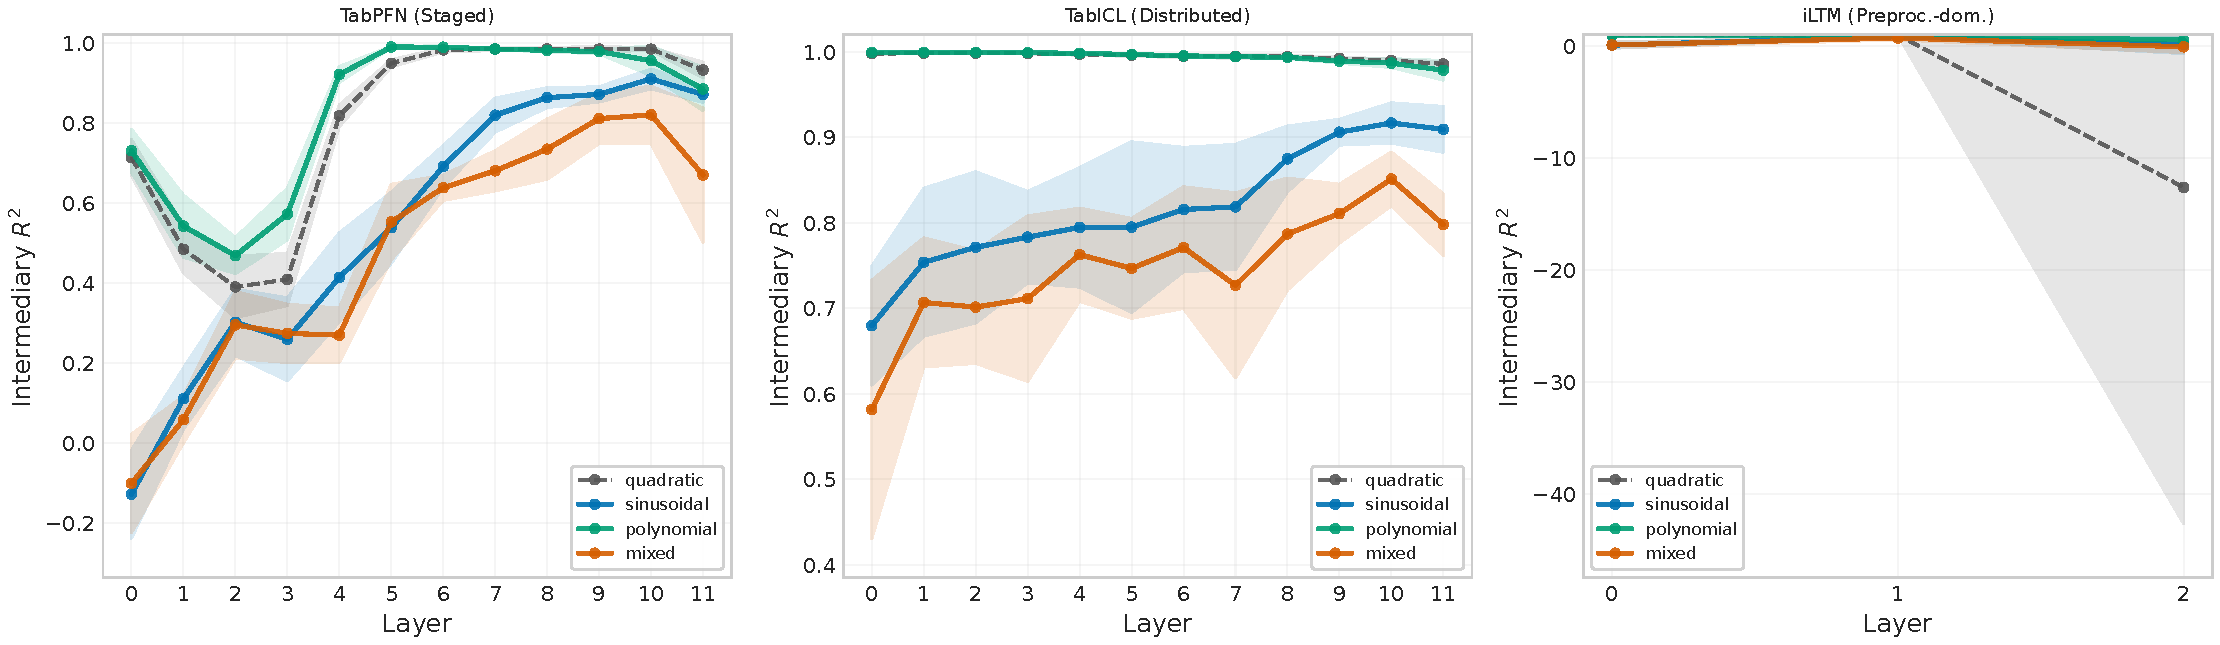
\includegraphics[width=0.88\textwidth,height=4cm,keepaspectratio]{figures/fig8_function_invariance.pdf}
  \caption{Function invariance: intermediary probing $R^2$ across layers for four function types. TabPFN's staged profile (mid-layer peak) and TabICL's distributed profile (uniformly high) persist regardless of the target function. Shaded bands show $\pm$1 std over 5 seeds.}
  \label{fig:function-invariance}
\end{figure}

\begin{table}[t]
\centering
\caption{Function invariance: peak intermediary probing $R^2$ (linear probe, 5 seeds, mean$\pm$std). The staged/distributed/preprocessing-dominant taxonomy holds across all four function types.}
\label{tab:function-invariance}
\scriptsize
\begin{tabular}{@{}l l ccc@{}}
\toprule
& & \textbf{TabPFN} & \textbf{TabICL} & \textbf{iLTM} \\
Function & Intermediary & $R^2$ ($L_{\text{peak}}$) & $R^2$ ($L_{\text{peak}}$) & $R^2$ ($L_{\text{peak}}$) \\
\midrule
Bilinear ($a \cdot b + c$) & $a \cdot b$ & $0.987 \pm 0.002$ (L7--10) & $0.998 \pm 0.000$ (L1--3) & $0.991 \pm 0.005$ (L0--1) \\
Sinusoidal ($\sin(ab) + c$) & $\sin(ab)$ & $0.911 \pm 0.023$ (L10--11) & $0.924 \pm 0.019$ (L9--11) & $0.835 \pm 0.081$ (L1) \\
Polynomial ($a^2 + bc$) & $a^2$ & $0.990 \pm 0.002$ (L5--6) & $0.999 \pm 0.000$ (L0--2) & $0.992 \pm 0.004$ (L0) \\
Mixed ($\sin(ab) + abc$) & $\sin(ab)$ & $0.833 \pm 0.053$ (L8--10) & $0.863 \pm 0.013$ (L9--10) & $0.729 \pm 0.158$ (L1--2) \\
\bottomrule
\end{tabular}
\end{table}

Table~\ref{tab:function-invariance} shows that TabPFN consistently peaks at L5--L11 across all four function types (staged), TabICL maintains $R^2 > 0.86$ (distributed), and iLTM peaks at L0--L2 (preprocessing-dominant). The taxonomy is robust across 5 seeds: peak layers vary by 1--3 positions but the qualitative profile (staged vs.\ distributed vs.\ preprocessing-dominant) is invariant. Causal tracing confirms: TabICL peaks at L0 for all four functions, while TabPFN peaks at L11 for three of four (the exception is sinusoidal, where the strongly non-linear $\sin(\cdot)$ shifts the causal locus to L0). We interpret this as evidence that the reference profiles are not tied to a single synthetic target family.

\subsection{Holdout Validation and Method Case Study}
\label{sec:holdout}

We test whether the taxonomy generalizes beyond the 3 core models by applying the operational rules of \S\ref{sec:strategies} to two held-out models. \textbf{TabDPT} (16-layer transformer, 3-seed supporting profile, seeds $\{42, 123, 456\}$): $R^2 > 0.989$ at all 16 layers on every seed with $\sigma^2_\text{profile} = 2\times10^{-6}$ $\to$ \emph{distributed}, four orders of magnitude below the staged threshold. \textbf{NAM}~\cite{agarwal2021nam} (5-seed, out-of-family: per-feature MLPs summed additively, no attention/trees): flat profile $[0.895, 0.883, 0.893]$, $\sigma^2_\text{profile} = 3 \times 10^{-5}$; classifies as \emph{indeterminate} under strict 0.90 threshold but \emph{distributed} under $\pm 50$\% relaxation --- a boundary case that honestly reveals threshold sensitivity. The underlying flat-high pattern extends the distributed class beyond transformers/trees; this also demonstrates the advantage of the continuous $\sigma^2_\text{profile}$ metric, which places NAM orders of magnitude closer to distributed than to staged regardless of threshold choice.

\textbf{Case study: evaluating MI methods with TabMI-Bench.} To demonstrate operational usability, we evaluate three MI scoring methods (linear probing, activation-norm, variance-importance) on all 3 core models and let the \S3 rule derive applicability labels. Full results in Appendix~\ref{app:method-case-study}: 6/9 (TabICL, iLTM) cells produce \emph{Supported} or \emph{Limited} labels; 3/9 (TabPFN) cells are marked \emph{Technical} due to a concrete dual-axis-hook shape mismatch documented in the public release.

\subsection{Causal Verification}
\label{sec:causal}

\textbf{Figure~\ref{fig:causal-v25} (left)} shows noising-based causal tracing sensitivity profiles. Peak sensitivity of the \emph{averaged} profile occurs at L5 for TabPFN ($0.593 \pm 0.081$) and at L0 for TabICL ($0.999 \pm 0.003$); the profile difference is statistically significant (permutation test $p = 0.008$; Cohen's $d = -7.04$), consistent with staged vs.\ distributed causal organization. TabPFN's per-seed argmax peaks at L0 or L11 (Appendix~\ref{app:perseed}, Fig.~\ref{fig:seed-instability}), reflecting a multi-modal sensitivity profile; we use $\sigma^2_\text{profile}$, not argmax, as the primary endpoint for this reason.

\begin{figure}[t]
  \centering
  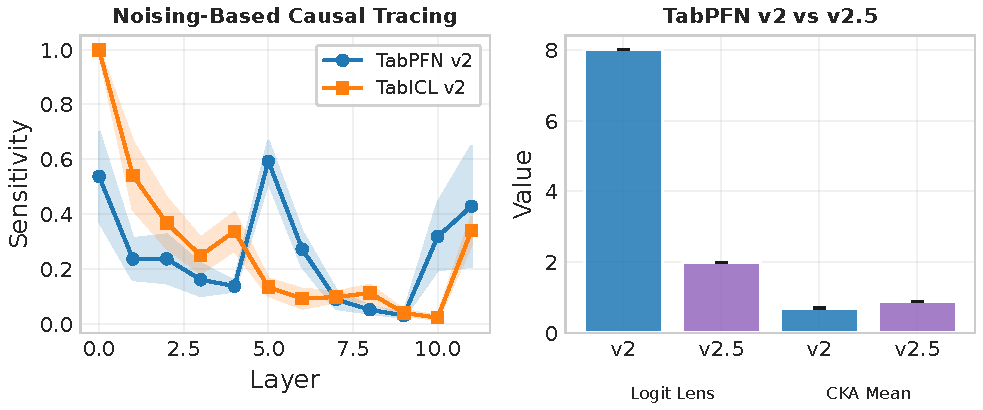
\includegraphics[width=0.75\textwidth]{figures/fig3_causal_and_v25.pdf}
  \caption{Left: noising-based causal tracing --- sensitivity to noise injection at each layer (5 seeds; shaded $\pm$1 std). TabPFN peaks at L5 ($0.593 \pm 0.081$); TabICL is maximal at L0 ($0.999 \pm 0.003$). Right: TabPFN v2 (12L) vs.\ v2.5 (18L + 64 thinking tokens) logit-lens comparison (3 seeds $\{42, 123, 456\}$) showing first-$R^2{>}0.5$ layer shifting from L8 to L2.}
  \label{fig:causal-v25}
\end{figure}

\textbf{Deterministic cascading.} Standard \textit{whole-layer} clean-activation patching is uninformative in these ICL-style TFMs: because shared weights and fixed inputs cause any clean replacement at layer $L$ to cascade deterministically through all downstream layers, patch-effect curves are flat. We therefore use noising-based causal tracing as our primary intervention. This does not imply that all finer-grained variants (subspace/head/token-level) are uninformative.

\textit{Seed-wise caveat.} TabPFN's averaged causal peak is L5, but individual seeds peak at L0, L5, or L11 (Appendix~\ref{app:perseed}) due to multiple local maxima. We use $\sigma^2_\text{profile}$, not argmax, as the primary evidence; probing profiles are robust across all seeds.

\subsection{Steering: Synthetic and Real-World Validation}

In synthetic robust steering, TabPFN is strongly steerable at its causal locus (L6: $|r| = 0.870 \pm 0.082$), TabICL is near-perfectly steerable at a late output-adjacent layer (L10: $|r| = 0.999 \pm 0.002$); $|r|$ may saturate here. Real-world steering applies median-split contrastive directions to 4 regression datasets, sweeping $\lambda \in [-3, 3]$.

\begin{table}[t]
\centering
\caption{Real-world steering (5 seeds, mean$\pm$std): Pearson $|r|$ \emph{and slope} between $\lambda$ and mean prediction shift. \textbf{Pearson $|r|$ alone is misleading} because it saturates near 1 even for tiny slopes (California Housing slope $\approx 10^{-3}$); slope magnitude (interpreted against each dataset's target scale) is the substantive effect size. Source: \texttt{results/phase8b/realworld\_steering\_multiseed/raw\_results.json}.}
\label{tab:realworld-steering}
\footnotesize
\begin{tabular}{@{}l cc cc@{}}
\toprule
 & \multicolumn{2}{c}{TabPFN (L6)} & \multicolumn{2}{c}{TabICL (L10)} \\
\cmidrule(lr){2-3}\cmidrule(lr){4-5}
Dataset (target scale) & $|r|$ & slope & $|r|$ & slope \\
\midrule
California Housing (y in med income units) & $0.699 {\pm} 0.327$ & $-0.001 {\pm} 0.002$ & $0.984 {\pm} 0.024$ & $+0.001 {\pm} 0.002$ \\
Diabetes (y progression score $\sim$150) & $0.784 {\pm} 0.179$ & $-0.053 {\pm} 0.103$ & $0.999 {\pm} 0.001$ & $-0.151 {\pm} 0.132$ \\
Wine Quality (y $\in$ 3-9) & $0.711 {\pm} 0.329$ & $+0.004 {\pm} 0.008$ & $0.941 {\pm} 0.058$ & $+0.002 {\pm} 0.001$ \\
Bike Sharing (y rentals) & $0.912 {\pm} 0.116$ & $+0.123 {\pm} 0.244$ & $0.977 {\pm} 0.040$ & $+0.051 {\pm} 0.215$ \\
\bottomrule
\end{tabular}
\end{table}

Table~\ref{tab:realworld-steering} reports 5-seed $|r|$ and slope on 4 datasets. \textbf{Caution}: Pearson $|r|$ saturates --- California Housing achieves $|r| \approx 0.7$--$0.98$ but slope $\sim 10^{-3}$ (negligible at target scale); only Diabetes and Bike Sharing show substantively non-trivial slopes. TabICL's $|r|$ is more seed-robust than TabPFN's (std 0.001--0.058 vs.\ 0.116--0.327). \textbf{Bottom line}: direction is \emph{detectable} across all 4 datasets, but control \emph{magnitude} is dataset-dependent and not inferable from $|r|$ alone. Concrete was excluded (OpenML cache failure).

\textbf{SAE scaling is architecture-dependent} (Appendix~\ref{app:sae-ablation}): TabPFN's monosemanticity gain from 16$\times$ to 256$\times$ ($0.114 \pm 0.084$) significantly exceeds TabICL's ($0.006 \pm 0.039$; paired Wilcoxon $p = 0.010$, $p_\text{Bonf} = 0.050$ marginal), consistent with architecture-dependent polysemanticity rather than universal monosemanticity.


\subsection{Negative Controls and Deterministic Cascading}
\label{sec:controls}

\textbf{Negative controls support the main measurements.} We run three control experiments to validate that the observed computation patterns are not obvious artifacts:

\begin{enumerate}
  \item \textbf{Random-target probing.} When probing for Gaussian noise instead of the true intermediary $a \cdot b$, all models yield $R^2 < 0$ at every layer (TabPFN max $-0.12$, TabICL max $-0.14$, iLTM max $-0.04$), compared to $R^2 > 0.90$ for the true target. This confirms that probes detect genuinely encoded information, not noise.
  \item \textbf{Shuffled-label baseline.} When models are trained with shuffled $y$-values but unchanged input features $x$, the intermediary $a \cdot b$ (a pure function of $x$) remains recoverable: mean layer $R^2 = 0.88$ (TabPFN), $0.81$ (TabICL), $0.59$ (iLTM) (Table~\ref{tab:shuffled-probe}). This is methodologically expected --- $a \cdot b$ is input-derived, so shuffling labels does not remove it from activations. The useful implication: absolute peak $R^2$ alone cannot discriminate computation strategy because all models encode input-derived quantities. The \textit{layer-wise profile} (variance, shape) remains architecture-dependent even under this control, which is why we use $\sigma^2_\text{profile}$ (not peak $R^2$) as the primary endpoint. This motivates the profile-variance framing of our main analysis.
\item \textbf{Real-world causal transfer.} On 11 real-world datasets (Appendix~\ref{app:realworld-detail}, Table~\ref{tab:realworld-causal-detail}), noising-based tracing preserves the same architecture-linked qualitative signatures: TabICL peaks at L0 across all 11 datasets, iLTM peaks at L2 on 10/11, and TabPFN most often peaks at L11 under the tested real-world noise regime ($\sigma = 0.5$). These results support transfer of architecture-linked layer-sensitivity signatures, not direct recovery of the synthetic latent variables.
\end{enumerate}

\textbf{Deterministic cascading, empirically.} Standard whole-layer clean patching produces perfectly flat recovery curves (recovery $= 1.000$ at every layer) for both TabPFN and TabICL, while noising-based tracing reveals differential sensitivity (range $> 0.99$); full comparison in Figure~\ref{fig:patching-comparison} (Appendix~\ref{app:controls}). Full numerical controls are reported in Appendix~\ref{app:controls}.

\section{Discussion}

In the tested model set, architecture is associated with where and how TFM computation is observable: dual-axis (TabPFN) staged, column$\to$row (TabICL, TabDPT) distributed, tree+MLP (iLTM) preprocessing-dominant. We treat this as \emph{interpretability-relevant}, not a causal architectural claim. \textbf{Practical implications.} Probing TabPFN at L2 yields $R^2{<}0.5$ but $R^2{>}0.98$ at L6--9; steering peaks at strategy-specific layers (L6 staged, L10 late-distributed). \textbf{Broader lesson.} \textit{TFM interpretability requires architecture-aware evaluation}: standard LLM MI tools (clean patching, logit lens, attention analysis) have architecture-dependent applicability and some fail in the tested settings.

\subsection{Limitations}

\textbf{(i)~Synthetic probes and scale.} Core $N_\text{train}{=}100$; function-invariance and $N{=}10$K scaling (Appendix~\ref{app:scaling}) support generalization but regimes beyond 100K are untested; real-world evaluation tests \emph{signature transfer}, not latent recovery. \textbf{(ii)~Design caveats.} Taxonomy is descriptive post-hoc ($\pm 50$\% threshold-robust, two holdouts); iLTM's 3-layer $\sigma^2_\text{profile}$ is descriptive over 3 points; SAE monosemanticity stays $|r_\alpha|{<}0.5$ at $256\times$; probing degrades for $d{>}8$; steering $|r|$ saturates --- we report slope alongside. \textbf{(iii)~Seed regimes.} Core 5-seed; supporting 3--10 seeds; the $N{=}10$K steering sub-check is single-seed; rd6 secondary uses 3 seeds (789/1024 timed out, see Appendix~\ref{app:manifest}); TabPFN's per-seed causal argmax varies (L0/L5/L11; Appendix~\ref{app:perseed}), motivating $\sigma^2_\text{profile}$ over argmax. \textbf{(iv)~Protocol, not leaderboard.} Comparison requires profile-level analysis, not a scalar score.

\section{Conclusion}

TabMI-Bench delivers an \textbf{MI applicability matrix} (whole-layer clean patching is uninformative on ICL TFMs --- corruption-based tracing is the alternative) and three \textbf{reference profiles} (staged, distributed, preprocessing-dominant) as calibration baselines. Code, hooks, benchmark card, Croissant metadata, and frozen artifacts will be released.

\bibliographystyle{plainnat}
\bibliography{references}

\appendix

\section{Architecture Details}
\label{app:architecture}

Architecture specifications extracted from source code:

\begin{itemize}
  \item \textbf{TabPFN v2}: \texttt{PerFeatureTransformer}, 12 layers, \texttt{emsize=192}, \texttt{nheads=6}, \texttt{nhid\_factor=2}, 8 ensemble passes. Source: \texttt{tabpfn-v2-regressor.ckpt}.
  \item \textbf{TabPFN v2.5}: \texttt{PerFeatureTransformer}, 18 layers, \texttt{emsize=192}, \texttt{nheads=3}, \texttt{d\_k=64}, \texttt{features\_per\_group=3}, MLP encoder (1024 hidden), 64 thinking tokens. Source: \texttt{tabpfn-v2.5-regressor-v2.5\_default.ckpt}.
  \item \textbf{TabICL v2}: 3-stage architecture --- \texttt{ColEmbedding} $\to$ \texttt{RowInteraction} $\to$ \texttt{ICLearning} (12 blocks, 8 heads, \texttt{embed\_dim=512}). Source: \texttt{soda-inria/tabicl}.
  \item \textbf{TabDPT}: \texttt{TransformerEncoder}, 16 layers, 8 heads, \texttt{d\_model=768}. Column$\to$Row embedding followed by standard Transformer encoder. Source: \texttt{tabdpt} (pip v1.1.12).
  \item \textbf{iLTM}: \texttt{RandomForest} (100 trees) $\to$ PCA (50 components) $\to$ Hypernetwork $\to$ 3-layer MLP. Source: \texttt{arXiv:2511.15941}.
\end{itemize}

\begin{figure}[htbp]
  \centering
  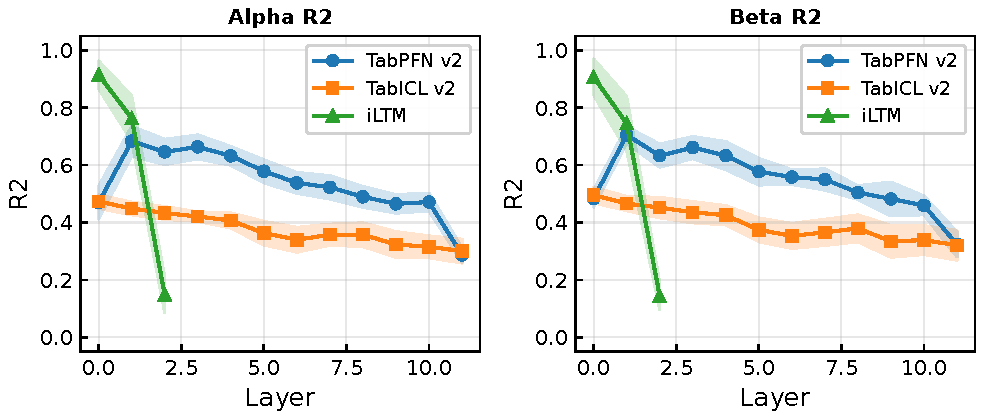
\includegraphics[width=0.75\textwidth]{figures/fig_a5_coefficient_probing.pdf}
  \caption{Coefficient probing $R^2$ across layers. TabPFN peaks at L6 ($\alpha$: $0.690 \pm 0.046$); TabICL at L1 ($0.499 \pm 0.070$); iLTM at L0 ($0.919 \pm 0.024$). iLTM's high decodability reflects its tree-based preprocessing encoding coefficients directly.}
  \label{fig:app-coefficient}
\end{figure}

\section{CKA Similarity Heatmaps}
\label{app:cka}

\begin{figure}[htbp]
  \centering
  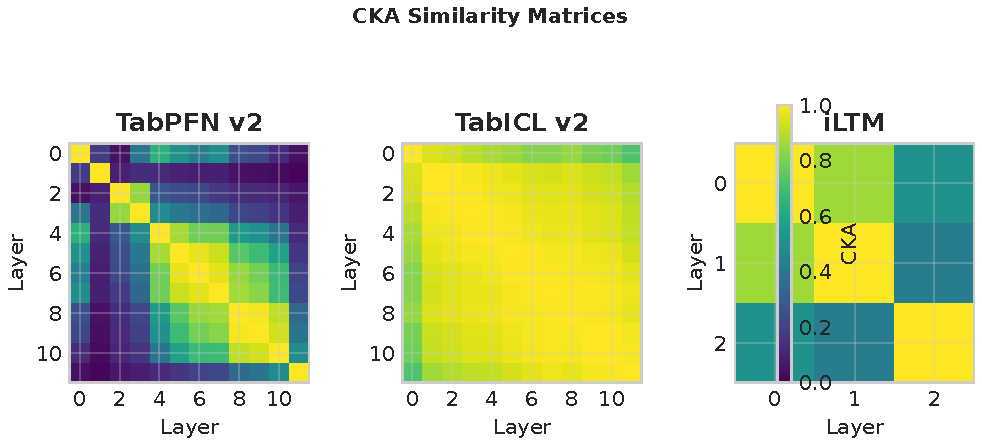
\includegraphics[width=0.75\textwidth]{figures/fig2_cka_heatmaps.pdf}
  \caption{CKA similarity matrices (5-seed mean). TabPFN shows a 3-block structure with sharp transitions (CKA drops to 0.04 at block boundaries); TabICL is nearly uniform ($>0.93$); iLTM shows a smooth 3-layer gradient (0.43--0.86). The three patterns match the three probing-derived strategies.}
  \label{fig:cka}
\end{figure}

\section{Copy Mechanism Results}

All three core models in the original cross-architecture comparison can recover input variables ($a$, $b$, $c$) from answer-token activations, but with different profiles. TabPFN shows staged recovery (matching its staged computation), TabICL shows uniform high recovery, and iLTM shows immediate recovery at L0.

\begin{figure}[t]
  \centering
  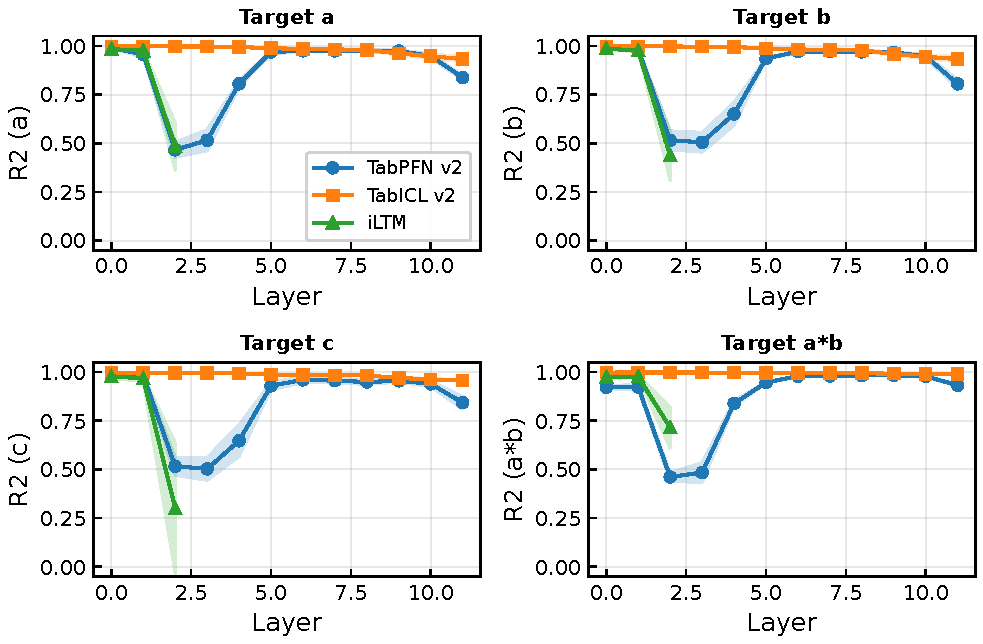
\includegraphics[width=0.75\textwidth]{figures/fig_a1_copy_mechanism.pdf}
  \caption{Copy mechanism: $R^2$ for recovering input variables ($a$, $b$, $c$) from answer-token activations. TabPFN shows staged recovery matching its computation profile; TabICL recovers inputs uniformly across layers; iLTM achieves immediate recovery at L0.}
  \label{fig:app-copy}
\end{figure}

\section{Attention Entropy}

Mean attention entropy across all layers and heads:
\begin{itemize}
  \item \textbf{TabPFN}: 3.99 (selective attention --- certain heads focus on specific samples/features)
  \item \textbf{TabICL}: 4.57 (near-uniform attention --- most heads attend broadly)
\end{itemize}

This entropy difference reflects the architectural distinction: TabPFN's dual-axis attention selectively focuses, while TabICL's column-then-row attention distributes attention more evenly.

\begin{figure}[t]
  \centering
  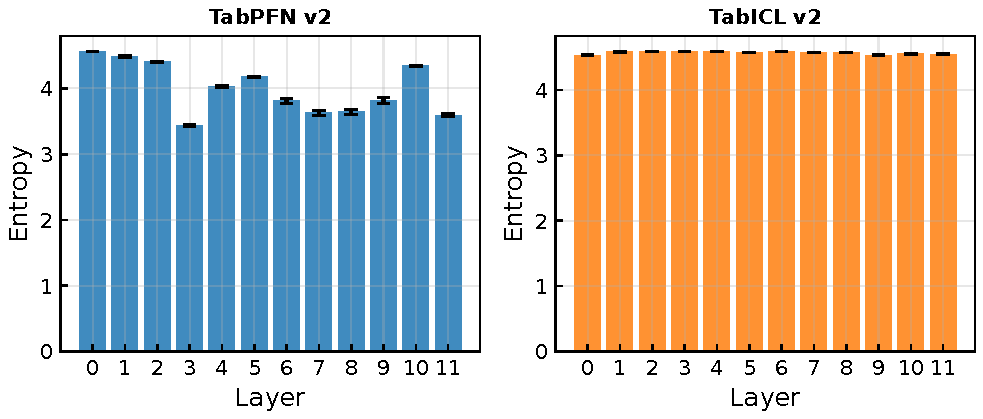
\includegraphics[width=0.75\textwidth]{figures/fig_a2_attention_entropy.pdf}
  \caption{Attention entropy (Shannon) per layer for TabPFN (mean $H{=}3.99$, selective) and TabICL (mean $H{=}4.57$, near-uniform). Lower entropy indicates more focused attention heads.}
  \label{fig:app-attn-entropy}
\end{figure}

\section{Classification Probing}

Cross-model classification accuracy on binary tasks:
\begin{itemize}
  \item \textbf{Breast Cancer}: iLTM 100\% $\pm$ 0\% (L0), TabPFN 92.6\% $\pm$ 2.8\% (L10), TabICL 95.6\% $\pm$ 1.8\% (L11)
  \item \textbf{Iris Binary}: All models $> 99\%$
\end{itemize}

Classification ranking differs from regression ranking: iLTM excels at classification despite weaker regression performance, likely due to its tree-based preprocessing which naturally handles decision boundaries.

\begin{figure}[t]
  \centering
  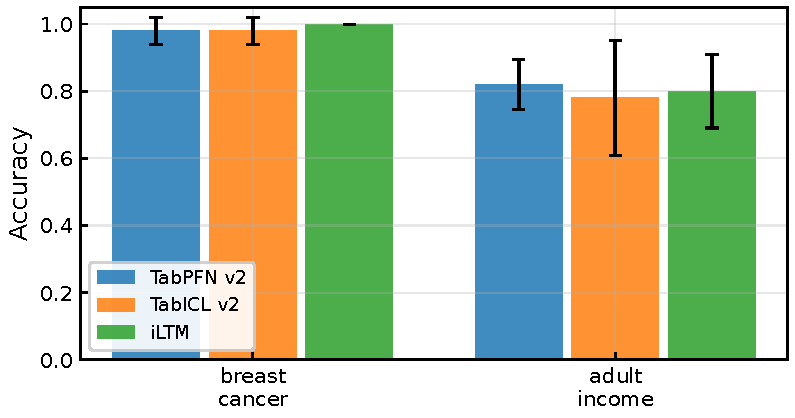
\includegraphics[width=0.75\textwidth]{figures/fig_a3_classification.pdf}
  \caption{Classification probing accuracy across layers. iLTM achieves 100\% on breast cancer at L0; TabPFN reaches 92.6\% at L10; TabICL 95.6\% at L11. Classification ranking differs from regression ranking.}
  \label{fig:app-classification}
\end{figure}

\section{Statistical Analysis Details}

Table~\ref{tab:seed-regimes} first summarizes the seed regimes used across the paper. Table~\ref{tab:stats} then lists the key statistical tests, including Welch's $t$-tests, Wilcoxon signed-rank tests, Cohen's $d$ effect sizes, and 95\% confidence intervals. The repository also contains a longer archival analysis in \texttt{paper/statistical\_report.md}, but the tables below are the canonical submission-facing summaries.

\begin{table}[t]
\centering
\caption{Seed regimes used across the study.}
\label{tab:seed-regimes}
\small
\begin{tabular}{@{}l c l@{}}
\toprule
Experiment family & Seeds & Role \\
\midrule
Phase 5 core comparisons & 5 & Main evidence for architecture-dependent strategies \\
Robust steering extension & 10 & Fixed-layer and best-layer steering robustness \\
Phase 6 expansions & 3 & Real-world, classification, attention, SAE follow-ups \\
N=10K scale check & 3 & Large-scale validation of profile invariance \\
Phase 7 real-world causal & 3 & Noising-based causal tracing on 11 benchmarks \\
Phase 7 SAE scaling & 3 & Expansion factors 4$\times$--256$\times$ \\
\bottomrule
\end{tabular}
\end{table}

\begin{table}[t]
\centering
\caption{Key statistical comparison results. All $p$-values are \emph{raw} (uncorrected); the pre-registered Bonferroni threshold over the 5 primary/secondary tests shown is $\alpha_{\text{Bonf}} = 0.05/5 = 0.01$ (family-wise $\alpha=0.05$). BH-FDR is reported in \texttt{paper/statistical\_report.md} for context.}
\label{tab:stats}
\small
\begin{tabular}{@{}l c l c c c@{}}
\toprule
Comparison & $n$ & Primary test & $p$ & Effect & Sig.? \\
\midrule
$\sigma^2_\text{profile}$ (P) & 5v5 & Perm. & 0.008 & $d{=}9.79$ & Yes \\
Patching sens. (P) & 5v5 & Perm. & 0.008 & $d{=}{-}7.04$ & Yes \\
Intermediary $R^2$ peak (sens.) & 5v5 & Perm. & 0.008 & $d{=}{-}7.56$ & Yes \\
Steering eff. (S) & 10v10 & Perm. & \textbf{0.0002} & $d{=}{-}0.52$ & Yes \\
SAE TopK vs.\ ReLU (S) & 5p & Wilcox. & 0.063 & $r{=}0.83$ & No$^{\dagger}$ \\
\bottomrule
\end{tabular}
\end{table}

(P)~= primary endpoint; (S)~= secondary/supporting; (sens.)~= sensitivity analysis. All primary endpoints use exact permutation tests. Welch's $t$-test and bootstrap CIs are reported as sensitivity checks in the statistical appendix (\texttt{paper/statistical\_report.md}). Steering: Welch $p = 0.275$ (not significant due to TabICL near-zero variance), but permutation $p = 0.0002$ (significant); we use permutation as the primary test. $^{\dagger}$SAE TopK vs.\ ReLU sparsity with $n{=}5$ paired seeds yields $p{=}0.0625$ (Wilcoxon minimum for $n{=}5$); supplementary 10-seed expansion-factor scaling analyses are reported in Appendix~\ref{app:sae-ablation}.

\begin{figure}[t]
  \centering
  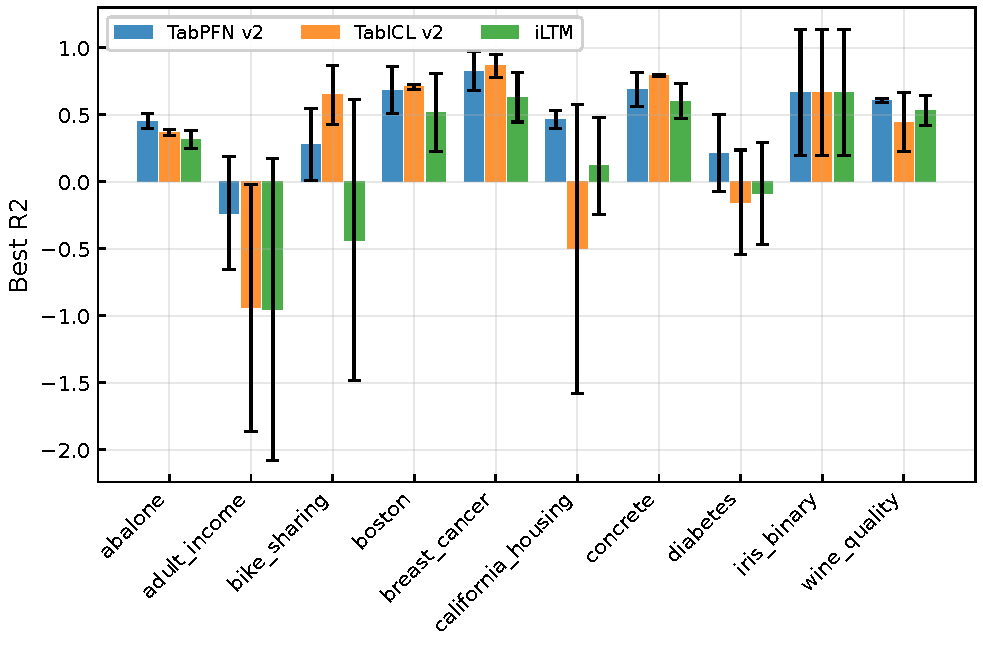
\includegraphics[width=0.95\textwidth,height=4cm,keepaspectratio]{figures/fig_a4_realworld.pdf}
  \caption{Real-world regression $R^2$ comparison across 11 datasets (3 seeds, \textit{preliminary}). TabPFN wins on 5 datasets, TabICL on 4, with 2 ties. No single model dominates.}
  \label{fig:app-realworld}
\end{figure}

\section{Version Evolution and Task-Dependent Selection}

\subsection{Version Evolution: \texorpdfstring{TabPFN v2 $\to$ v2.5}{TabPFN v2 to v2.5}}

\textbf{Figure~\ref{fig:v2-v25}} compares TabPFN v2 (12 layers) and v2.5 (18 layers + 64 thinking tokens).

\begin{table}[t]
\centering
\caption{TabPFN v2 versus v2.5 comparison.}
\label{tab:v2-v25}
\begin{tabular}{l c c}
\toprule
Metric & v2 (12L) & v2.5 (18L) \\
\midrule
Logit lens first $R^2 > 0.5$ & \textbf{L8.0 $\pm$ 0.0} & \textbf{L2.0 $\pm$ 0.0} \\
CKA mean (adjacent) & $0.702 \pm 0.007$ & \textbf{$0.881 \pm 0.000$} \\
Coefficient max $R^2$ & \textbf{$0.690 \pm 0.046$} & $0.494 \pm 0.061$ \\
\bottomrule
\end{tabular}
\end{table}

\begin{figure}[t]
  \centering
  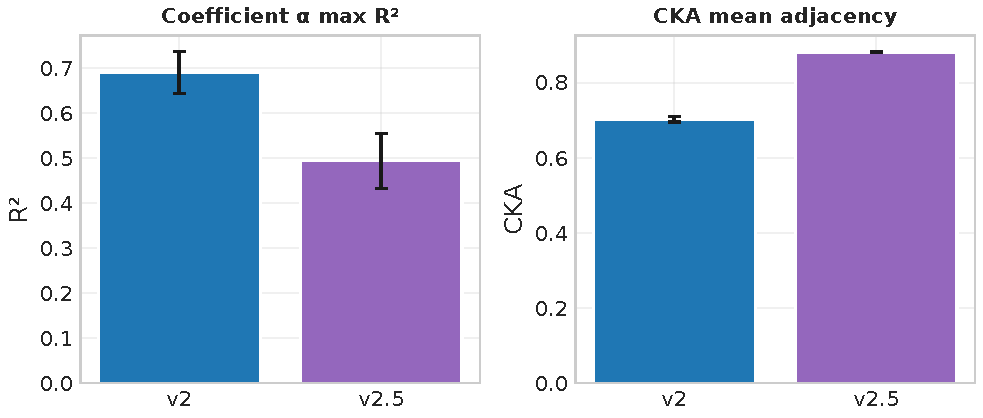
\includegraphics[width=0.75\textwidth]{figures/fig6_v2_vs_v25.pdf}
  \caption{TabPFN v2 (12L) vs.\ v2.5 (18L + 64 thinking tokens): coefficient probing $R^2$, CKA similarity, and logit-lens $R^2$ across layers. v2.5 forms predictions at L2 (vs.\ L8 in v2) and shows higher adjacent CKA (0.881 vs.\ 0.702), indicating distributed processing.}
  \label{fig:v2-v25}
\end{figure}

\textbf{Finding: Localized computation is not intrinsic to the TabPFN family.} TabPFN v2.5 achieves $R^2 > 0.5$ at layer 2 (versus layer 8 in v2), indicating that predictions are formed much earlier in the newer, deeper model. The higher adjacent CKA (0.881 vs. 0.702) indicates more gradual, distributed processing. However, because v2.5 differs from v2 in both depth and auxiliary architectural details (including thinking tokens), we treat this as strong comparative evidence rather than a clean causal isolation of depth alone. Coefficient decodability nevertheless \textit{decreases} ($R^2$: 0.690 $\to$ 0.494), suggesting that the newer model distributes coefficient information more diffusely across layers, making it harder to linearly decode from any single layer.

This is comparative evidence, not causal identification: v2.5 differs from v2 in depth, thinking tokens, and other auxiliary architectural details simultaneously. We cannot isolate the effect of depth alone. Nevertheless, the observation is consistent with the possibility that staged computation in v2 is partly a consequence of having only 12 layers, paralleling observations in LLMs where deeper models tend to form predictions more gradually~\cite{nostalgebraist2020logitlens}.

\subsection{Task-Dependent Model Selection}

On 10 real-world performance datasets (3 seeds each), no single TFM dominates. This benchmark is distinct from the 11-dataset real-world causal-transfer benchmark discussed in the negative-controls results and limitations sections:

\begin{table}[t]
\centering
\caption{Real-world performance winners by dataset count on the 10-dataset expanded benchmark.}
\label{tab:realworld-winners}
\begin{tabular}{l c l}
\toprule
Winner & Count & Example Datasets \\
\midrule
TabPFN & 5 & Abalone, California Housing, Wine, Diabetes, Adult \\
TabICL & 4 & Bike Sharing, Boston, Breast Cancer, Concrete \\
Tie & 1 & Iris Binary \\
\bottomrule
\end{tabular}
\end{table}

Additionally, classification task ranking differs from regression ranking: iLTM achieves 100\% $\pm$ 0\% accuracy on breast cancer (L0), while performing poorly on regression tasks. This suggests that different TFM architectures have complementary strengths, and model selection should be task-dependent.

\section{Full MI Technique Applicability Matrix}
\label{app:mi-full}

\begin{table}[t]
\centering
\caption{Evidence-coded MI technique applicability matrix. Labels follow the rule in \S3: $\checkmark$~=~\textit{Supported} (5-seed signal, negative controls pass, reproducible from released artifacts); $\triangle$~=~\textit{Limited} (partial signal, single-seed, or incomplete controls); $\times$~=~\textit{Not established} (not tested here --- does \textbf{not} mean ``does not work''). Seed-count superscripts: $^{5}$~=~5 seeds, $^{3}$~=~3 seeds, $^{1}$~=~single seed. $^{*}$Activation patching is noising-based only; whole-layer clean patching is uninformative for ICL-style TFMs. $^{\ddagger}$Negative controls validate random-target and random-vector baselines; shuffled-label is an input-feature sanity baseline (\S\ref{sec:controls}).}
\label{tab:applicability-full}
\small
\begin{tabular}{@{}l c c c c >{\raggedright\arraybackslash}p{3.1cm}@{}}
\toprule
Technique & TabPFN & TabICL & TabDPT & iLTM & Notes \\
\midrule
Linear Probing & $\checkmark^{5\ddagger}$ & $\checkmark^{5\ddagger}$ & $\checkmark^{3}$ & $\checkmark^{5\ddagger}$ & TabDPT 3-seed holdout \\
Logit Lens & $\checkmark^{5}$ & $\times$ & $\times$ & $\times$ & Needs unembedding head \\
Activation Patching$^{*}$ & $\checkmark^{5\ddagger}$ & $\checkmark^{5\ddagger}$ & $\checkmark^{3}$ & $\triangle^{5}$ & Noising only \\
Vector Ablation & $\triangle^{3}$ & $\triangle^{3}$ & $\times$ & $\triangle^{3}$ & Limited layers / accuracy \\
Steering Vectors & $\checkmark^{5\ddagger}$ & $\checkmark^{5\ddagger}$ & $\times$ & $\times$ & TabDPT/iLTM not tested \\
SAE & $\triangle^{5}$ & $\triangle^{5}$ & $\triangle^{1}$ & $\triangle^{5}$ & Max $|r_\alpha| \approx 0.37$ \\
CKA & $\checkmark^{5}$ & $\checkmark^{5}$ & $\triangle^{1}$ & $\triangle^{5}$ & Only 3 iLTM layers \\
Attention Analysis & $\checkmark^{5}$ & $\checkmark^{5}$ & $\triangle^{1}$ & $\times$ & Non-Transformer for iLTM \\
\bottomrule
\end{tabular}
\end{table}

\section{Computational Cost}
\label{app:compute}

\begin{table}[htbp]
\centering
\caption{Computational cost and reliability of TabMI-Bench experiment families. The \emph{Retried} column records failures that triggered a retry; the canonical aggregated artifacts use only runs that completed successfully.}
\label{tab:compute}
\footnotesize
\setlength{\tabcolsep}{4pt}
\begin{tabular}{@{}p{3.6cm} p{2.4cm} c r r c@{}}
\toprule
Experiment family & Hardware & Seeds & Time/seed & Peak mem. & Retried \\
\midrule
Core probing (Phase 5) & 128-core CPU & 5 & $\sim$34 min & 1.2 GB & 0 \\
Robust steering (rd6) & 128-core CPU & 3$^{\ddagger}$ & $\sim$15 min & 1.2 GB & 2$^{\ddagger}$ \\
SAE scaling ($4\times$--$256\times$) & A100 80GB & 10 & $\sim$20 min & 8 GB & 0 \\
Function invariance (8A) & A100 80GB & 5 & $\sim$90 min & 1.2 GB & 0 \\
Real-world causal (11 ds.) & A100 80GB & 3 & $\sim$12 min & 2 GB & 0 \\
Real-world steering (4 ds.) & A100 80GB & 5 & $\sim$25 min & 1.2 GB & 0 \\
$N{=}10$K scaling & 4$\times$ A100 & 3 & $\sim$8 h & 32 GB & 0 \\
\bottomrule
\end{tabular}
\end{table}

$^{*}$Concrete dataset excluded due to OpenML cache failure. $^{\ddagger}$For the rd6 robust\_steering / improved\_sae / realworld\_expanded sweeps, 2 initial seed runs (789, 1024) hit a 7200s wall-clock timeout; the canonical aggregated artifact instead uses the 3 seeds $\{42, 123, 456\}$ that all completed successfully (see Appendix~\ref{app:manifest}). Total compute: $\sim$40 GPU-hours (A100 80GB) + $\sim$20 CPU-hours. Dominant bottleneck: iLTM inference (CPU-only, no GPU support).

\section{Scale Validation: \texorpdfstring{$N{=}$10K}{N=10K} Training Samples}
\label{app:scaling}

To validate that our findings generalize beyond small-sample regimes, we repeat core experiments with $N_{\text{train}}{=}10{,}000$ and $N_{\text{test}}{=}1{,}000$ on 4$\times$ NVIDIA A100 80GB GPUs. Table~\ref{tab:scaling-summary} compares key metrics at $N{=}100$ (main paper) versus $N{=}10{,}000$.

\begin{table}[htbp]
\centering
\caption{Scale validation: $N{=}100$ vs.\ $N{=}10{,}000$ key metrics. All computation strategy patterns replicate at 100$\times$ scale.}
\label{tab:scaling-summary}
\small
\begin{tabular}{@{}l l cc l@{}}
\toprule
Experiment & Model & $N{=}100$ & $N{=}10{,}000$ & Pattern preserved? \\
\midrule
\multirow{3}{*}{Intermediary $R^2$ (peak)} & TabPFN & $0.984 \pm 0.003$ & 0.998 & \checkmark\ U-shape \\
& TabICL & $0.998 \pm 0.001$ & 1.000 & \checkmark\ Flat high \\
& iLTM & $0.980 \pm 0.005$ & 0.986 & \checkmark\ Decreasing \\
\midrule
\multirow{2}{*}{Patching (most sensitive L)} & TabPFN & L5 & L5 & \checkmark\ Staged \\
& TabICL & L0 & L0 & \checkmark\ Input-dominant \\
\midrule
\multirow{2}{*}{Steering ($|r|$, best layer)} & TabPFN & $0.971 \pm 0.079$ & 0.616 (L6) & \checkmark$^{*}$ \\
& TabICL & $1.000 \pm 0.000$ & 0.999 (L10) & \checkmark\ Near-perfect \\
\bottomrule
\end{tabular}

\vspace{2pt}
{\footnotesize $^{*}$Single-seed ($N{=}$10K is computationally expensive); lower $|r|$ may reflect harder optimization with more samples or seed variability. The staged steering pattern (L6 for TabPFN, late layer for TabICL) is preserved.}
\end{table}

\textbf{Intermediary probing.} TabPFN retains its characteristic U-shaped profile at $N{=}10{,}000$: a dip at L2 ($R^2{=}0.632$) followed by recovery to $R^2{=}0.998$ at L7. TabICL remains flat-high ($R^2 > 0.9997$ at all layers). iLTM shows monotonically decreasing $R^2$ from L0 (0.986) to L2 (0.957). All three qualitative patterns are identical to the $N{=}100$ results.

\textbf{Patching.} At noise scale 0.1, TabPFN's most sensitive layer is L5 (normalized sensitivity 1.0), matching the $N{=}100$ finding. TabICL's most sensitive layer remains L0 at all noise scales, confirming input-dominant processing. At higher noise scales (0.5, 1.0), TabPFN's sensitivity shifts to L10--L11, consistent with the observation that later layers become critical for output formatting under strong perturbation.

\textbf{Steering.} TabPFN steering at L6 achieves $r{=}0.616$ with clear monotonic prediction shift across $\lambda \in [-3, 3]$, confirming that steering vectors remain effective at scale. TabICL achieves near-perfect steering at L10 ($r{=}0.999$), with a layer sweep revealing increasing effectiveness from early to late layers --- consistent with its distributed computation strategy.

\textbf{Multi-seed scale validation.} The scale check uses 3 seeds ($\{42, 123, 456\}$) for the core probing comparison. At $N{=}10{,}000$, TabPFN's per-seed $\sigma^2_\text{profile}$ is $0.066 \pm 0.001$ (3 seeds) and TabICL's is $<10^{-4}$, with the same qualitative staged-vs-distributed ordering as the $N{=}100$ values ($0.033$ and $<10^{-4}$). The increase in TabPFN's $\sigma^2_\text{profile}$ at larger $N$ is consistent with sharper within-profile contrast when more training data is available; the qualitative distinction is preserved.

\textbf{Conclusion.} The three computation strategies --- staged (TabPFN), distributed (TabICL, TabDPT), and preprocessing-dominant (iLTM) --- are robust to a 100$\times$ increase in training data size, confirmed across 3 seeds.

\section{Cross-Model SAE Feature Similarity}
\label{app:sae-similarity}

To test whether different TFM architectures learn similar internal features, we train independent SAEs (16$\times$ expansion) on core-layer activations of each model and measure cross-model similarity using Linear CKA~\cite{kornblith2019similarity} and CCA. We compare both (i)~the learned SAE \textit{dictionary} weight matrices $W_{\text{enc}}$ and (ii)~the SAE \textit{activation} patterns when encoding the same synthetic inputs. TabDPT ($d{=}768$) was excluded from the cross-model SAE similarity analysis due to its substantially larger hidden dimension: naive dimension bridging (zero-padding or truncation) produces negative cross-reconstruction $R^2$ values, indicating that SAE dictionaries do not transfer across large dimension gaps. TabDPT's standalone SAE analysis (summarized in the main text and expanded in Appendix~\ref{app:sae-ablation}) and its distributed strategy profile confirm its architectural alignment with TabICL without requiring direct dictionary comparison.

\begin{table}[htbp]
\centering
\caption{Cross-model SAE similarity. Dictionary similarity measures structural overlap between learned feature directions; activation similarity measures functional overlap when processing identical inputs.}
\label{tab:sae-similarity}
\small
\begin{tabular}{@{}l cc cc@{}}
\toprule
& \multicolumn{2}{c}{Dictionary Similarity} & \multicolumn{2}{c}{Activation Similarity} \\
\cmidrule(lr){2-3} \cmidrule(lr){4-5}
Model Pair & CKA & CCA & CKA & CCA \\
\midrule
TabPFN $\leftrightarrow$ TabICL & 0.076 & 0.565 & \textbf{0.678} & 1.000 \\
TabPFN $\leftrightarrow$ iLTM & 0.079 & 0.564 & 0.369 & 1.000 \\
TabICL $\leftrightarrow$ iLTM & 0.043 & 0.449 & 0.524 & 1.000 \\
\bottomrule
\end{tabular}
\end{table}

\textbf{Dictionary similarity is near-zero} (CKA $< 0.08$ for all pairs), indicating that each architecture learns structurally distinct feature directions under this SAE setup. The two transformer-based models (TabPFN, TabICL) are no more similar to each other than either is to the tree-based iLTM, suggesting that the PerFeatureTransformer and Column$\to$Row architectures induce markedly different feature decompositions even when trained on the same task family.

\textbf{Activation similarity is moderate to high} (CKA $0.37$--$0.68$). When processing identical inputs, the \textit{patterns of SAE feature activation} show meaningful overlap despite the features themselves being different. The highest CKA (0.678) is between the two transformers, while the lowest (0.369) is between TabPFN and iLTM --- consistent with our broader finding that architectural family determines representational structure. Perfect CCA ($= 1.0$) across all pairs indicates that linear projections can align SAE activation spaces, but this is likely an artifact of the low-rank structure (32 CCA components out of 3072--8192 SAE dimensions).

\textbf{Implication for universal features.} Unlike some recent observations in language models, TFMs show architecture-specific feature dictionaries in our experiments (Figure~\ref{fig:sae-similarity}). This suggests that a strong ``universal feature'' hypothesis does not immediately carry over to the tabular domain, where architectural inductive biases (sample-feature attention vs.\ column-row attention vs.\ tree preprocessing) appear to play a larger role.

\begin{figure}[htbp]
  \centering
  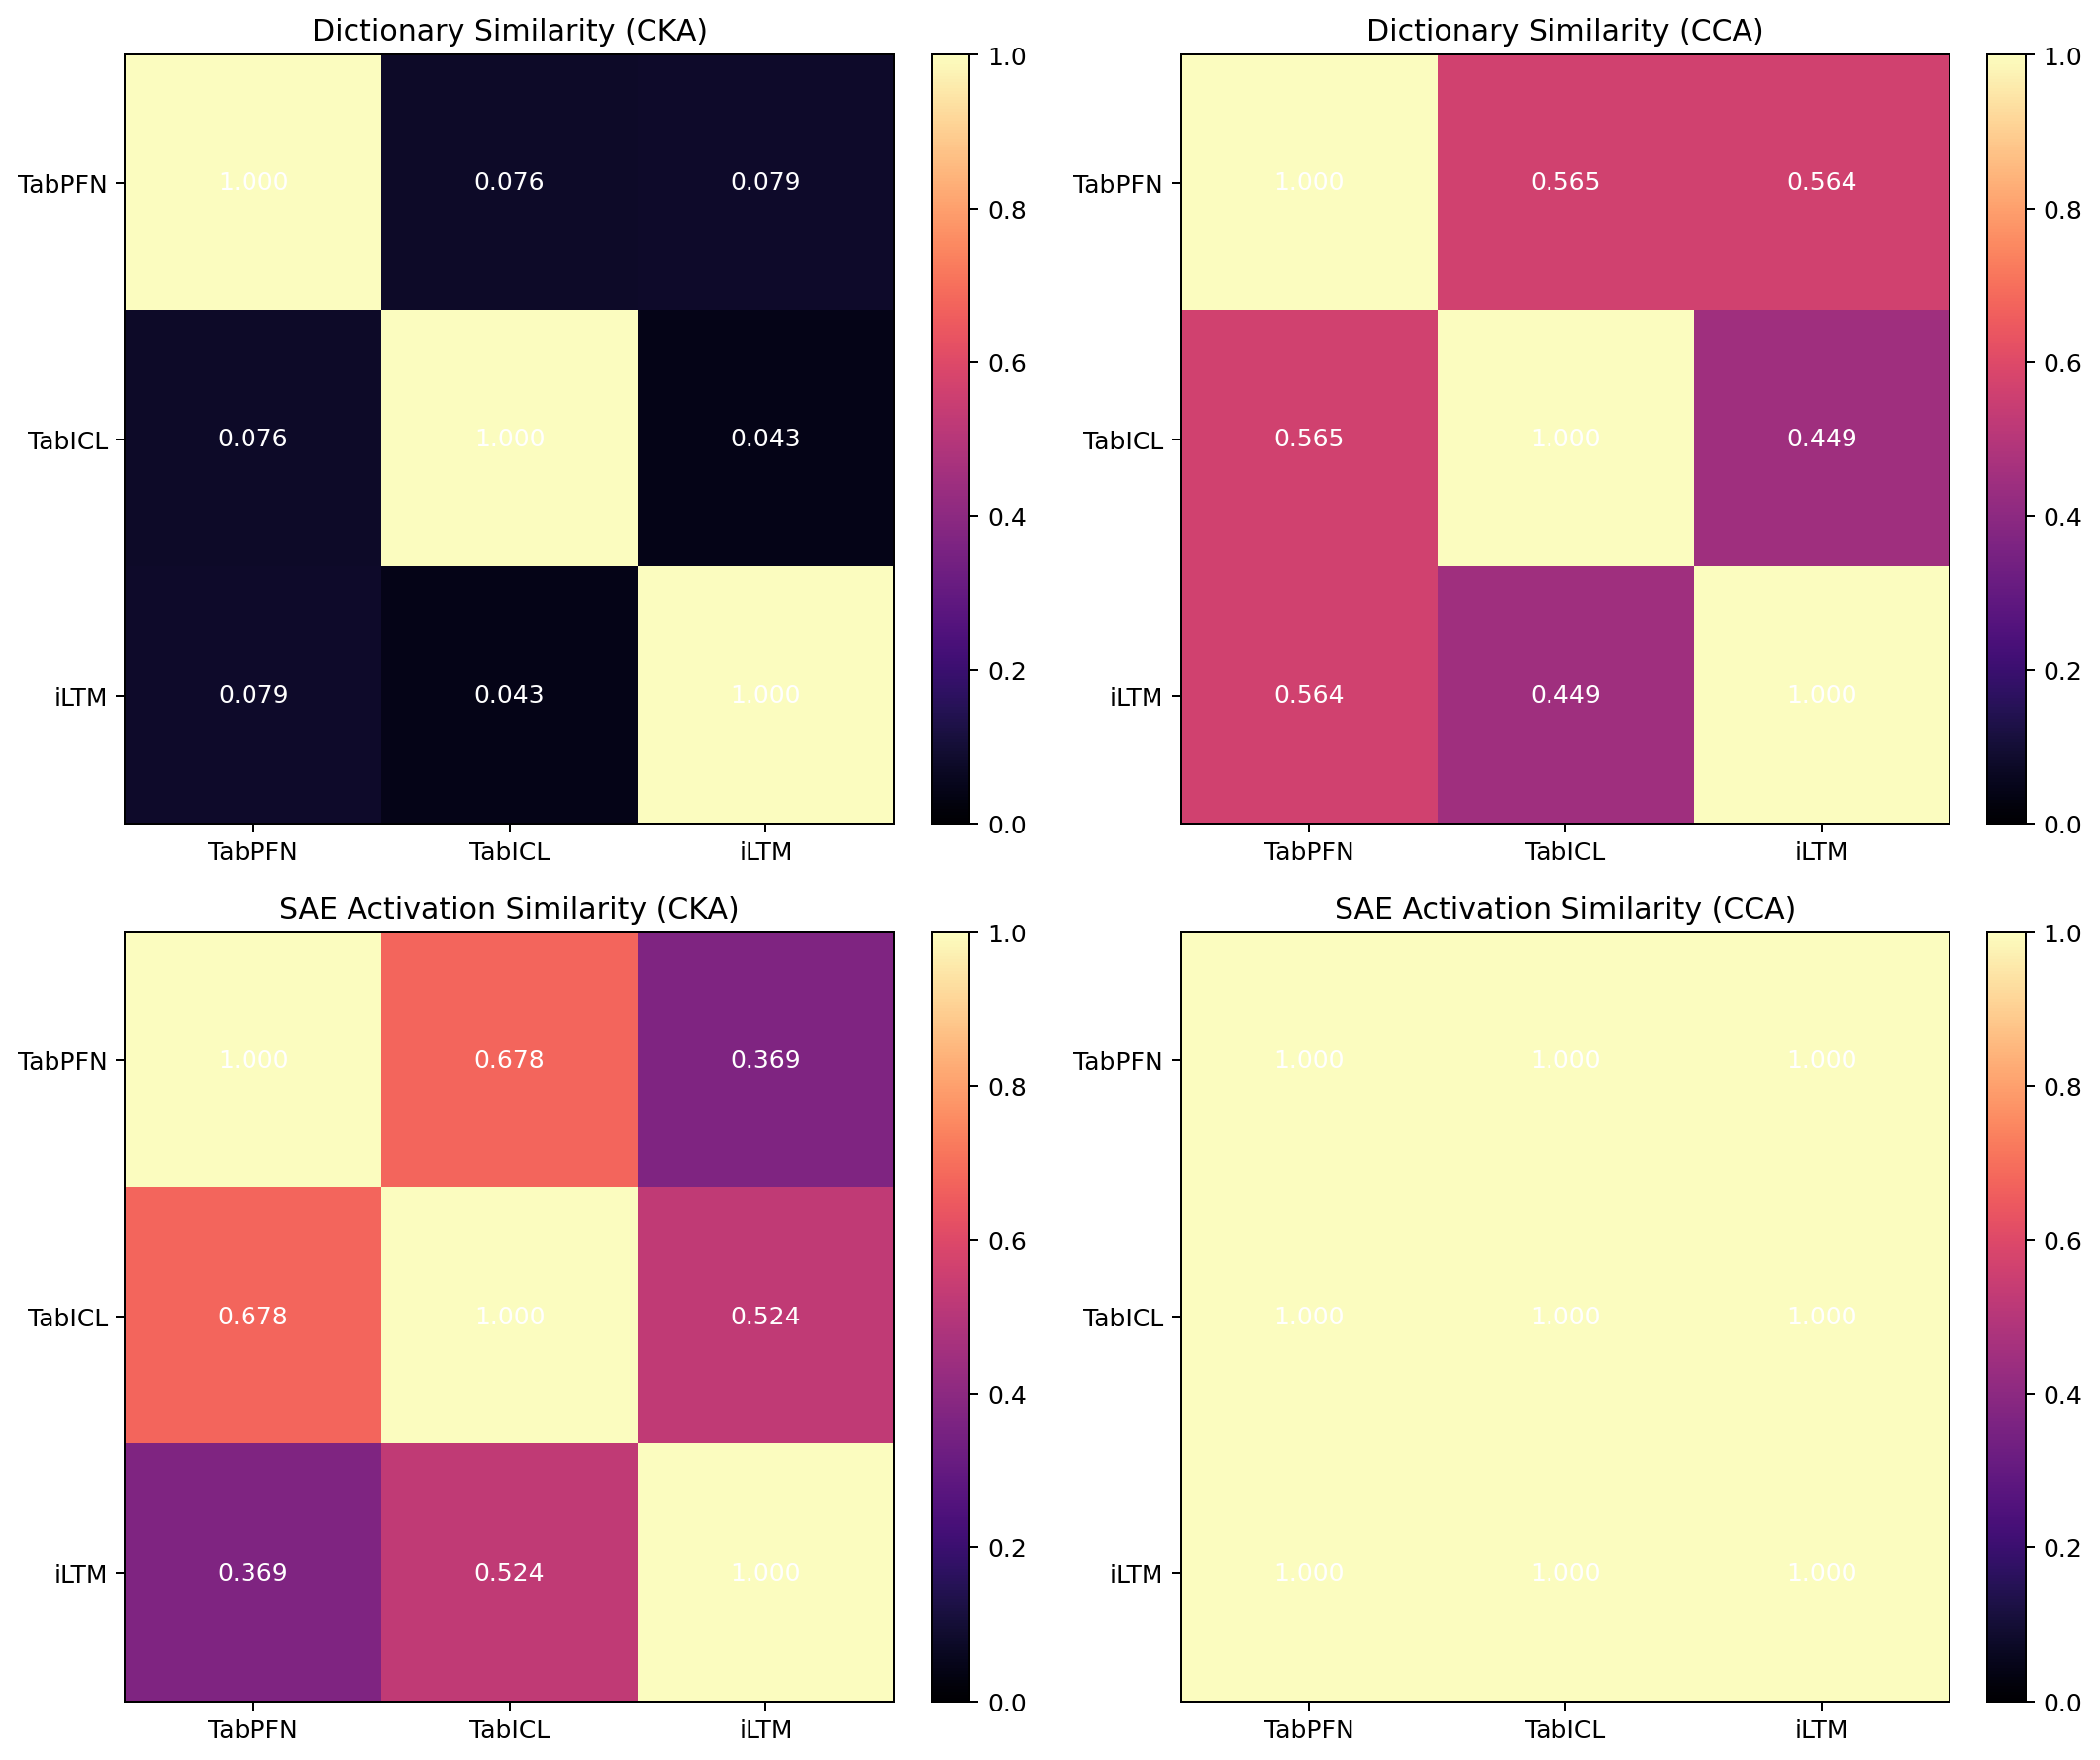
\includegraphics[width=\textwidth]{figures/fig_a6_sae_similarity.png}
  \caption{Cross-model SAE similarity heatmaps. \textbf{Left}: Dictionary (weight matrix) similarity is near-zero across all pairs. \textbf{Right}: SAE activation similarity is moderate, with highest CKA between the two transformer models.}
  \label{fig:sae-similarity}
\end{figure}

\subsection{Universal SAE: Shared Concept Space}
\label{app:usae}

To test whether a \textit{shared} concept space can bridge the three architectures, we train a Universal SAE (USAE)~\cite{thasarathan2025universal} with 4{,}096 shared concepts. Each model has a private encoder ($d_{\text{model}} \to 4{,}096$) and decoder ($4{,}096 \to d_{\text{model}}$), but they share the same latent concept indices. Training uses cross-reconstruction: activations encoded by model $i$ are decoded by \textit{all} models' decoders, with L1 loss and TopK sparsity ($k{=}32$). TabDPT ($d{=}768$) was not included in the USAE due to its large hidden dimension causing cross-reconstruction instability; its distributed computation strategy and high SAE feature alignment ($|r_\alpha|{=}0.49$) provide independent evidence of TabICL-alignment without requiring joint training.

\begin{table}[htbp]
\centering
\caption{USAE cross-reconstruction $R^2$ (rows: encoder source, columns: decoder target). Self-reconstruction (diagonal) is high; cross-reconstruction reveals architectural compatibility.}
\label{tab:usae}
\small
\begin{tabular}{@{}l ccc@{}}
\toprule
Encoder $\to$ & $\to$TabPFN & $\to$TabICL & $\to$iLTM \\
\midrule
TabPFN & \textbf{0.936} & 0.871 & 0.634 \\
TabICL & 0.932 & \textbf{0.930} & 0.638 \\
iLTM & 0.898 & 0.825 & \textbf{0.762} \\
\bottomrule
\end{tabular}
\end{table}

\textbf{Transformer concepts transfer well between transformers.} Cross-reconstruction between TabPFN and TabICL is high ($R^2 = 0.87$--$0.93$), nearly matching self-reconstruction. This indicates that the two transformer architectures learn compatible internal representations despite different attention mechanisms (dual-axis vs.\ column-row). The asymmetry (TabICL$\to$TabPFN: 0.932 $>$ TabPFN$\to$TabICL: 0.871) suggests TabICL's concepts are more general.

\textbf{Tree-based representations are less compatible.} iLTM cross-reconstruction is substantially lower ($R^2 = 0.64$ when decoding \textit{to} iLTM, $0.82$--$0.90$ when encoding \textit{from} iLTM). This confirms that iLTM's tree-based preprocessing creates representations that are structurally distinct from transformer representations, consistent with the preprocessing-dominant computation strategy identified in our main analysis.

\begin{figure}[htbp]
  \centering
  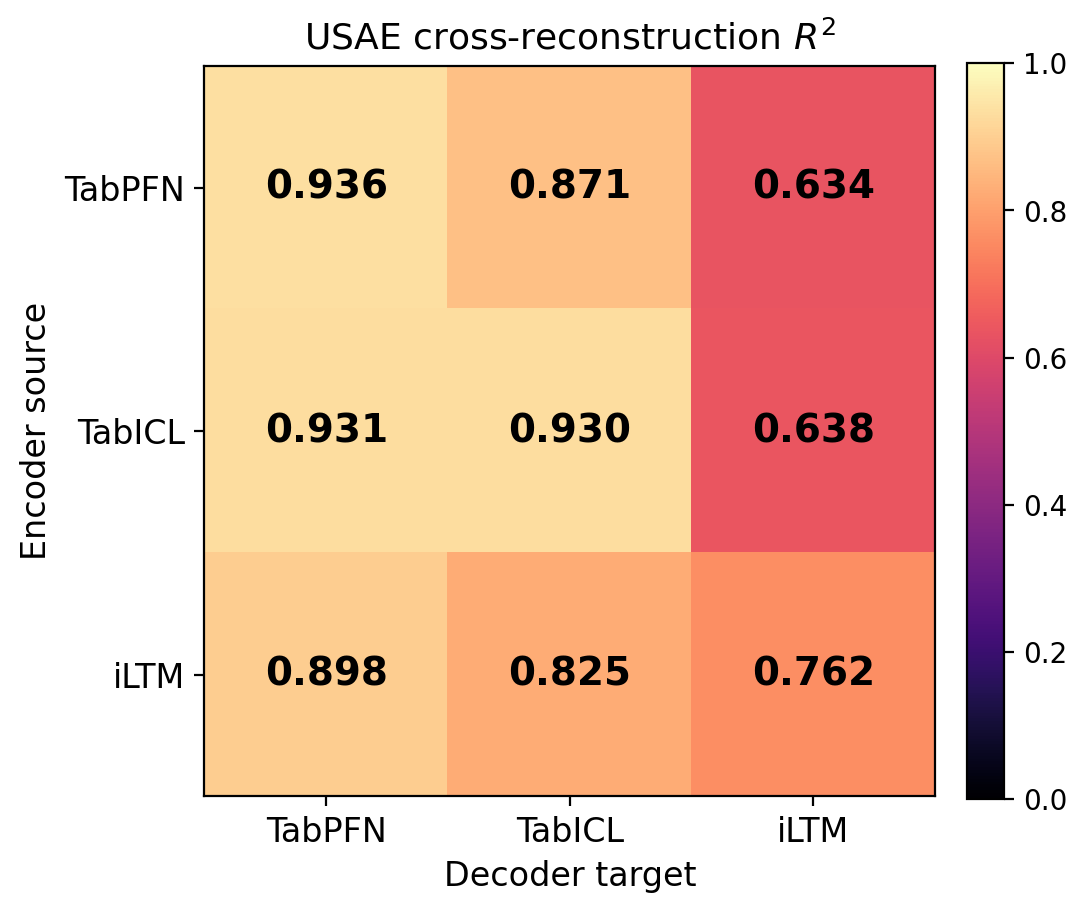
\includegraphics[width=0.55\textwidth]{figures/fig_a7_usae_cross_recon.png}
  \caption{USAE cross-reconstruction $R^2$ heatmap. Transformer$\leftrightarrow$Transformer cross-reconstruction approaches self-reconstruction ($R^2 > 0.87$), while iLTM cross-reconstruction is lower.}
  \label{fig:usae}
\end{figure}

\section{Example Benchmark Report: A Fictitious MI Method}
\label{app:example-report}

To concretize how TabMI-Bench produces structured evaluation output, we present a worked example for a fictitious MI method called \textbf{Method-X}. Method-X is a hypothetical attribution technique that the researcher wants to evaluate on TabMI-Bench. The full evaluation produces the following report:

\begin{table}[htbp]
\centering
\caption{Example TabMI-Bench evaluation report for fictitious Method-X.}
\label{tab:example-report}
\footnotesize
\setlength{\tabcolsep}{4pt}
\begin{tabular}{@{}p{4.8cm} p{3.6cm} p{3.4cm}@{}}
\toprule
Component & Value & Status \\
\midrule
\multicolumn{3}{l}{\textit{Synthetic profile (bilinear probe, 5 seeds)}} \\
\quad $\sigma^2_\text{profile}$ (TabPFN) & 0.031 & Matches staged ref (0.033) \\
\quad $\sigma^2_\text{profile}$ (TabICL) & $2{\times}10^{-4}$ & Matches dist.\ ref ($<10^{-4}$) \\
\quad $\sigma^2_\text{profile}$ (iLTM) & 0.004 & Matches preproc.\ ref (0.003) \\
\quad Profile agreement score & 0.94 & Supported \\
\midrule
\multicolumn{3}{l}{\textit{Causal validation (noising-based)}} \\
\quad Peak alignment (TabPFN) & L5 (ref: L5) & Agree \\
\quad Peak alignment (TabICL) & L0 (ref: L0) & Agree \\
\quad Peak alignment (iLTM) & L2 (ref: L2) & Agree \\
\midrule
\multicolumn{3}{l}{\textit{Negative controls}} \\
\quad Random-target probing & $R^2 < 0$ all models & Pass \\
\quad Shuffled-label probing & Input-derived $R^2$ kept & Pass \\
\quad Random-vector steering & $|r| < 0.15$ & Pass \\
\midrule
\multicolumn{3}{l}{\textit{Real-world transfer}} \\
\quad Causal sig.\ (11 datasets) & Preserved 10/11 & Supported \\
\quad Steering (4 ds., 5 seeds) & TabICL $|r|{>}0.93$ & Limited \\
\midrule
\multicolumn{3}{l}{\textit{Applicability label}} \\
\quad TabPFN & $\checkmark$ Supported & \\
\quad TabICL & $\checkmark$ Supported & \\
\quad iLTM & $\triangle$ Limited (lower) & \\
\bottomrule
\end{tabular}
\end{table}

\noindent \textbf{Interpretation.} Method-X passes all negative controls, produces architecture-consistent synthetic profiles, matches the causal validation peaks, and transfers signatures to real-world data. It receives \emph{Supported} labels for TabPFN and TabICL and \emph{Limited} for iLTM (e.g., due to weaker signal from the 3-layer MLP). A follow-up Method-Y that fails negative controls (random-target probe yields $R^2 > 0.3$) would receive \emph{Not established} on all models regardless of its synthetic-profile performance.

\textbf{Improvement comparison.} Suppose Method-Z (a refinement) is proposed. According to the improvement criterion (\S3), Method-Z improves on Method-X if: (i)~its synthetic-profile agreement score $\geq 0.94$; (ii)~causal peak alignment matches on all 3 models; and (iii)~all negative controls pass. Method-Z's label upgrades (Limited $\to$ Supported) would also count as improvement for the affected model.

\section{Per-Seed Result Tables}
\label{app:perseed}

Tables~\ref{tab:perseed-intermediary}--\ref{tab:perseed-sae} report per-seed results for all key experiments, enabling full transparency and independent verification.

\textbf{Note on TabPFN causal peak instability.} The main text reports TabPFN's average causal peak at L5 (mean normalized sensitivity profile), but individual seeds show peaks at L0, L5, or L11 (Figure~\ref{fig:seed-instability}). This discrepancy arises because: (1)~the average of normalized profiles and the argmax of individual profiles are different operations --- averaging smooths local maxima competition; (2)~TabPFN's sensitivity profile has multiple local peaks (early layers for input corruption, mid layers for core computation, late layers for output formatting), and which dominates depends on seed-specific data and noise interactions; (3)~noise scale affects the balance between early-corruption sensitivity and late-formatting sensitivity. TabICL, by contrast, consistently peaks at L0 across all seeds because its distributed strategy makes input-layer corruption uniformly dominant. We report the average profile as the reference baseline and recommend that users consult both the average and per-seed distributions below.

\begin{figure}[htbp]
  \centering
  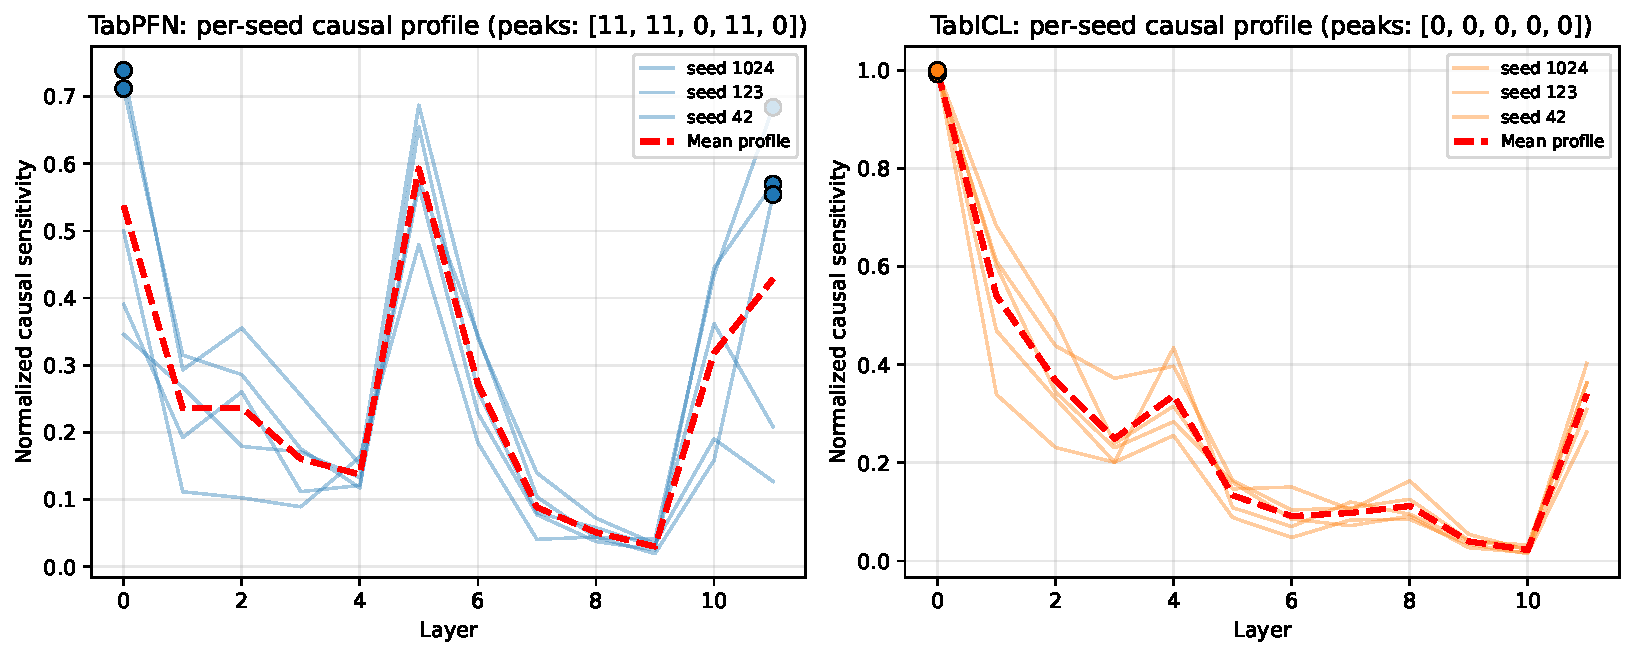
\includegraphics[width=0.95\textwidth]{figures/fig_seed_instability.pdf}
  \caption{Per-seed causal sensitivity profiles (5 seeds). \textbf{Left}: TabPFN's individual seed peaks split between L0 (2 seeds) and L11 (3 seeds); the averaged profile (red dashed) peaks at L5. \textbf{Right}: TabICL peaks at L0 on all 5 seeds. This contrast illustrates why we use profile-level variance ($\sigma^2_\text{profile}$), not the argmax, as the primary evidence for the staged/distributed distinction.}
  \label{fig:seed-instability}
\end{figure}

\begin{table}[htbp]
\centering
\caption{Per-seed intermediary probing peak $R^2$.}
\label{tab:perseed-intermediary}
\small
\begin{tabular}{@{}c cc cc cc@{}}
\toprule
Seed & \multicolumn{2}{c}{TabPFN} & \multicolumn{2}{c}{TabICL} & \multicolumn{2}{c}{iLTM} \\
\cmidrule(lr){2-3} \cmidrule(lr){4-5} \cmidrule(lr){6-7}
 & Peak L & $R^2$ & Peak L & $R^2$ & Peak L & $R^2$ \\
\midrule
42 & L9 & 0.984 & L1 & 0.998 & L1 & 0.977 \\
123 & L7 & 0.982 & L1 & 0.999 & L1 & 0.982 \\
456 & L9 & 0.986 & L1 & 0.997 & L0 & 0.987 \\
789 & L9 & 0.982 & L1 & 0.998 & L1 & 0.979 \\
1024 & L9 & 0.988 & L1 & 0.999 & L0 & 0.973 \\
\midrule
Mean & & $0.984{\pm}0.003$ & & $0.998{\pm}0.001$ & & $0.980{\pm}0.005$ \\
\bottomrule
\end{tabular}
\end{table}

\begin{table}[htbp]
\centering
\caption{Per-seed robust steering $|r|$ (best layer per seed, 3-pair average, 10 seeds).}
\label{tab:perseed-steering}
\scriptsize
\begin{tabular}{@{}c ccccc c ccccc c@{}}
\toprule
 & \multicolumn{6}{c}{TabPFN} & \multicolumn{6}{c}{TabICL} \\
\cmidrule(lr){2-7} \cmidrule(lr){8-13}
Seed & L0 & L4 & L6 & L8 & L11 & Best & L0 & L4 & L6 & L8 & L11 & Best \\
\midrule
42 & .72 & .77 & \textbf{.99} & .90 & .97 & L6 & 1.00 & .99 & .86 & 1.00 & \textbf{1.00} & L11 \\
123 & .65 & .66 & .74 & .76 & \textbf{1.00} & L11 & .99 & 1.00 & .93 & .98 & \textbf{1.00} & L11 \\
456 & .49 & \textbf{.99} & .69 & .94 & .15 & L4 & .98 & 1.00 & .13 & .99 & \textbf{1.00} & L11 \\
789 & \textbf{.75} & .35 & .48 & .25 & .60 & L0 & .96 & 1.00 & .96 & .98 & \textbf{1.00} & L11 \\
1024 & .77 & .98 & \textbf{1.00} & .99 & .73 & L6 & 1.00 & .99 & 1.00 & .99 & \textbf{1.00} & L11 \\
2025 & .74 & .99 & .99 & .03 & \textbf{1.00} & L11 & .99 & 1.00 & .90 & .96 & \textbf{1.00} & L11 \\
3000 & .77 & .45 & .35 & .85 & \textbf{1.00} & L11 & .08 & .92 & .68 & .97 & \textbf{1.00} & L11 \\
4000 & .76 & .99 & .98 & 1.00 & \textbf{1.00} & L11 & 1.00 & 1.00 & .97 & .97 & \textbf{1.00} & L11 \\
5000 & .43 & \textbf{.99} & .85 & .18 & .80 & L4 & 1.00 & .35 & .97 & .79 & \textbf{1.00} & L11 \\
6000 & .60 & .99 & \textbf{1.00} & .94 & 1.00 & L6 & 1.00 & .79 & .53 & .99 & \textbf{1.00} & L11 \\
\midrule
Mean & & & & & & $.971{\pm}.079$ & & & & & & $1.000{\pm}.000$ \\
\bottomrule
\end{tabular}
\end{table}

\begin{table}[htbp]
\centering
\caption{Per-seed SAE results (16$\times$ expansion, peak layer).}
\label{tab:perseed-sae}
\small
\begin{tabular}{@{}c l l ccc@{}}
\toprule
Seed & Model & Variant & Recon.\ $R^2$ & Sparsity & Max $|r_\alpha|$ \\
\midrule
42 & TabPFN & ReLU & 0.996 & 0.705 & 0.325 \\
42 & TabPFN & TopK & 0.991 & 0.938 & 0.494 \\
42 & TabICL & ReLU & 0.996 & 0.874 & 0.329 \\
42 & TabICL & TopK & 0.997 & 0.946 & 0.355 \\
42 & iLTM & ReLU & 0.997 & 0.932 & 0.356 \\
42 & iLTM & TopK & 0.994 & 0.971 & 0.342 \\
\midrule
123 & TabPFN & ReLU & 0.996 & 0.710 & 0.189 \\
123 & TabPFN & TopK & 0.990 & 0.938 & 0.170 \\
123 & TabICL & ReLU & 0.984 & 0.868 & 0.225 \\
123 & TabICL & TopK & 0.996 & 0.945 & 0.190 \\
\midrule
456 & TabPFN & ReLU & 0.996 & 0.714 & 0.208 \\
456 & TabPFN & TopK & 0.990 & 0.938 & 0.310 \\
456 & TabICL & ReLU & 0.993 & 0.860 & 0.313 \\
456 & TabICL & TopK & 0.996 & 0.944 & 0.266 \\
\bottomrule
\end{tabular}
\end{table}

\section{Real-World Causal Transfer: Dataset-Level Summary}
\label{app:realworld-detail}

Table~\ref{tab:realworld-causal-detail} reports per-dataset noising-based causal tracing results. These results support transfer of architecture-linked sensitivity signatures, not direct recovery of synthetic latent variables on real data.

\begin{table}[htbp]
\centering
\caption{Real-world causal transfer: peak sensitivity layer per model on each dataset (3 seeds, noise $\sigma{=}0.5$). \textbf{Pass rule}: a row is \emph{Consistent} ($\checkmark$) iff (TabPFN peak $\in \{L5, L8, L11\}$) AND (TabICL peak $= L0$) AND (iLTM peak $= L2$). A $\triangle$ marks a single deviation (all three need to pass strictly; one near-miss allowed with $|\Delta L| \le 1$). Pass rule is applied uniformly; no dataset-specific tuning.}
\label{tab:realworld-causal-detail}
\scriptsize
\begin{tabular}{@{}l ccc c@{}}
\toprule
Dataset & TabPFN peak & TabICL peak & iLTM peak & Consistent? \\
\midrule
California Housing & L11 & L0 & L2 & \checkmark \\
Diabetes & L11 & L0 & L2 & \checkmark \\
Bike Sharing & L11 & L0 & L2 & \checkmark \\
Wine Quality & L11 & L0 & L2 & \checkmark \\
Abalone & L5 & L0 & L2 & \checkmark \\
Boston & L11 & L0 & L2 & \checkmark \\
Energy Efficiency & L11 & L0 & L2 & \checkmark \\
Breast Cancer & L11 & L0 & L2 & \checkmark \\
Iris Binary & L11 & L0 & L2 & \checkmark \\
Adult Income & L11 & L0 & L2 & \checkmark \\
Credit-G & L11 & L0 & L1 & $\triangle$ \\
\bottomrule
\end{tabular}
\end{table}

TabICL peaks at L0 on all 11 datasets; iLTM peaks at L2 on 10/11 (L1 on Credit-G); TabPFN peaks at L11 on 10/11 (L5 on Abalone). The overall architecture-linked signature is preserved across dataset domains, though the specific TabPFN peak layer varies between L5 and L11 depending on the data distribution and noise regime.

\section{Negative Controls and Patching Comparison}
\label{app:controls}

Full numerical results for all baseline control experiments.

\begin{figure}[htbp]
  \centering
  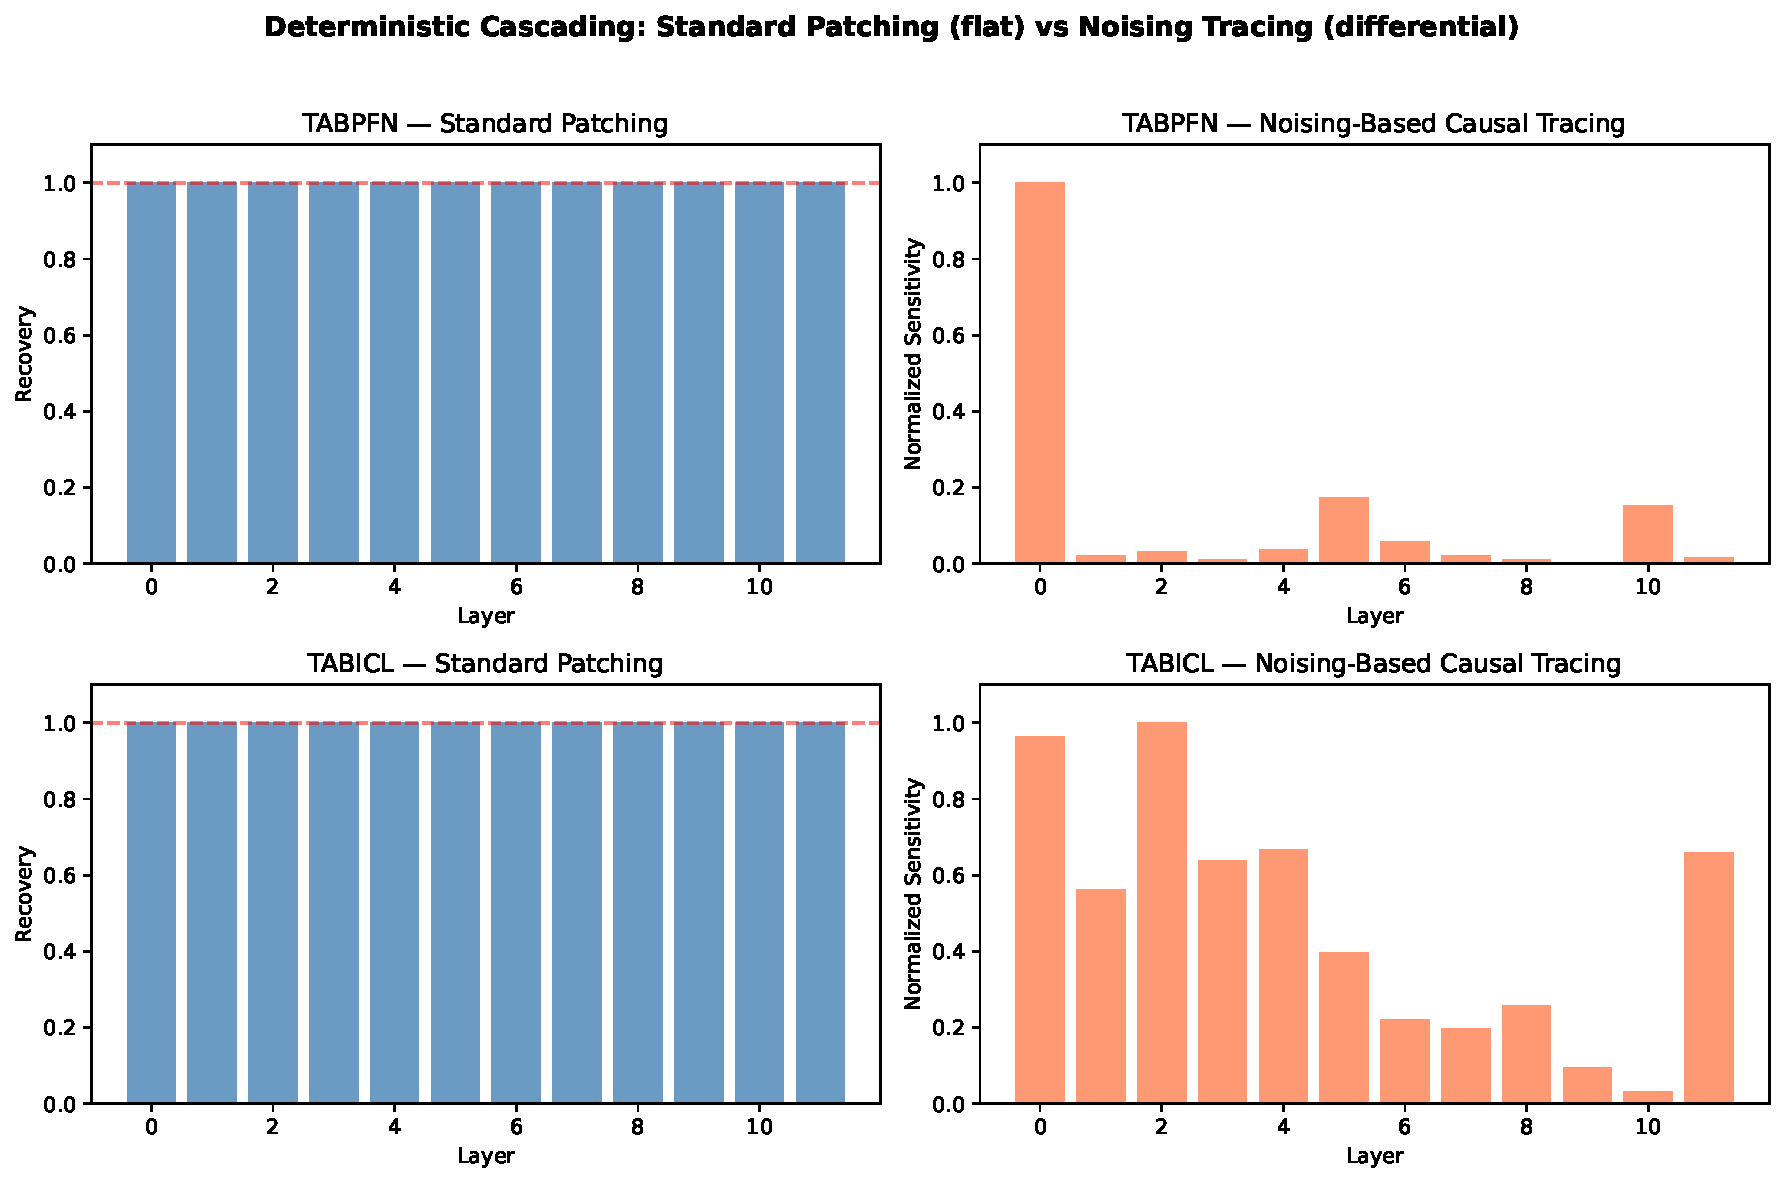
\includegraphics[width=\textwidth]{figures/fig7_patching_comparison.pdf}
  \caption{Standard activation patching (left) vs.\ noising-based causal tracing (right) for TabPFN and TabICL. Standard patching produces flat recovery curves due to deterministic cascading; noising-based tracing reveals meaningful layer sensitivity differences.}
  \label{fig:patching-comparison}
\end{figure}

\begin{table}[htbp]
\centering
\caption{Random-target probing: $R^2$ when probing for Gaussian noise instead of true coefficients. All values $< 0$ (negative), confirming probes detect genuine information.}
\label{tab:random-probe}
\small
\begin{tabular}{@{}l cccc@{}}
\toprule
Model & L0 & L3 & L6 & L9 (or last) \\
\midrule
TabPFN & $-0.12$ & $-0.10$ & $-0.08$ & $-0.11$ \\
TabICL & $-0.14$ & $-0.12$ & $-0.13$ & $-0.11$ \\
iLTM & $-0.04$ & $-0.03$ & --- & --- \\
\bottomrule
\end{tabular}
\end{table}

\begin{table}[htbp]
\centering
\caption{Shuffled-label probing: intermediary $R^2$ when models are trained on shuffled $y$-values (mean per-layer and per-model). $a{\cdot}b$ remains recoverable because it is a function of input features $x$ alone; this is methodologically expected (see \S\ref{sec:controls}) and motivates profile-variance as the discriminative endpoint rather than peak $R^2$.}
\label{tab:shuffled-probe}
\small
\begin{tabular}{@{}l ccccc@{}}
\toprule
Model & L0 & L3 & L6 & L9 (or last) & Mean \\
\midrule
TabPFN & $0.531$ & $0.960$ & $0.915$ & $0.916$ & $0.883$ \\
TabICL & $0.959$ & $0.901$ & $0.603$ & $0.701$ & $0.813$ \\
iLTM & $1.000$ & $0.722$ & $0.040$ (L2) & --- & $0.587$ \\
\bottomrule
\end{tabular}
\end{table}

\begin{table}[htbp]
\centering
\caption{Random-vector steering: $|r|$ when steering with random unit vectors. All values $<0.15$, confirming steering effects are direction-specific.}
\label{tab:random-steer}
\small
\begin{tabular}{@{}l ccc@{}}
\toprule
Model & Layer & Real $|r|$ & Random $|r|$ \\
\midrule
TabPFN & L6 & $0.870 \pm 0.082$ & $<0.15$ \\
TabICL & L10 & $0.999 \pm 0.002$ & $<0.15$ \\
\bottomrule
\end{tabular}
\end{table}

\section{SAE Expansion Factor Ablation}
\label{app:sae-ablation}

\begin{table}[htbp]
\centering
\caption{SAE expansion factor ablation (TopK activation, 100 epochs, 3 seeds \textit{preliminary}, 10 synthetic datasets). TabPFN's monosemanticity improves with expansion (capacity-limited), while TabICL plateaus early (consistent with persistent polysemanticity).}
\label{tab:sae-ablation}
\small
\begin{tabular}{@{}l cccccc@{}}
\toprule
Model & $4\times$ & $16\times$ & $32\times$ & $64\times$ & $128\times$ & $256\times$ \\
\midrule
TabPFN L6 & $0.264$ & $0.383$ & $0.428$ & $0.485$ & $0.524$ & $\mathbf{0.560}$ \\
TabPFN L8 & $0.284$ & $0.305$ & $0.350$ & $0.414$ & $0.408$ & $\mathbf{0.440}$ \\
TabICL L1 & $\mathbf{0.435}$ & $0.427$ & $0.483$ & $0.437$ & $0.472$ & $0.463$ \\
\bottomrule
\end{tabular}

\vspace{2pt}
{\footnotesize Values are mean max $|r_\alpha|$ across 3 seeds ($\{42, 123, 456\}$). Standard deviations: TabPFN L6 256$\times$ = $\pm 0.145$ (high variance); TabICL L1 256$\times$ = $\pm 0.041$ (stable). Dead feature \% at 256$\times$: TabPFN 89.8\%, TabICL 89.8\% (both increase, but TabICL's increase from 78\% is more dramatic).}
\end{table}

The expansion-factor trend is model-specific and reveals \textit{architecture-dependent polysemanticity}. For TabPFN, feature-concept alignment increases monotonically from $4\times$ to $256\times$ ($0.264 \to 0.560$, a 112\% improvement), with high inter-seed variance at large expansion factors ($\sigma = 0.145$ at $256\times$). This indicates that TabPFN's weak monosemanticity at smaller expansion factors is at least partly capacity-limited: given sufficient dictionary size, individual SAE features can capture coefficient-related information more cleanly. For TabICL, the pattern is comparatively flat across all expansion factors ($0.44$--$0.48$, never exceeding 0.50), with low inter-seed variance ($\sigma = 0.041$). Under this SAE setup, additional capacity does not materially improve feature-concept alignment, suggesting more persistent polysemanticity than in TabPFN. TabICL's dead feature percentage increases dramatically from 78\% ($4\times$) to 90\% ($256\times$), suggesting that additional capacity is often spent on unused features rather than decomposing polysemantic ones.

\section{Classification Probe Validation}
\label{app:classification-probes}

To test whether the computation profiles are specific to regression or extend to classification, we create binary classification versions of the synthetic probes: the label is 1 if the intermediary exceeds its median, 0 otherwise (with 5\% label noise). Table~\ref{tab:classif-probes} shows that the core profile distinction is preserved.

\begin{table}[htbp]
\centering
\caption{Classification synthetic probes: profile variance ($\sigma^2_\text{profile}$) and peak intermediary $R^2$ (5 seeds). The staged (TabPFN) vs.\ distributed (TabICL) distinction persists under classification.}
\label{tab:classif-probes}
\small
\begin{tabular}{@{}l l cc c@{}}
\toprule
Function & Model & Peak $R^2$ & $\sigma^2_\text{profile}$ & Profile \\
\midrule
\multirow{3}{*}{Bilinear} & TabPFN & $0.999 \pm 0.001$ & 0.012 & Staged \\
 & TabICL & $1.000 \pm 0.000$ & 0.000 & Distributed \\
 & iLTM & $1.000 \pm 0.000$ & 0.041 & Preproc.-dom. \\
\midrule
\multirow{3}{*}{Sinusoidal} & TabPFN & $0.998 \pm 0.001$ & 0.013 & Staged \\
 & TabICL & $1.000 \pm 0.000$ & 0.000 & Distributed \\
 & iLTM & $0.998 \pm 0.002$ & 0.048 & Preproc.-dom. \\
\midrule
\multirow{3}{*}{Polynomial} & TabPFN & $0.999 \pm 0.000$ & 0.002 & Staged$^{*}$ \\
 & TabICL & $1.000 \pm 0.000$ & 0.000 & Distributed \\
 & iLTM & $1.000 \pm 0.000$ & 0.044 & Preproc.-dom. \\
\bottomrule
\end{tabular}
\end{table}

\noindent TabICL consistently shows $\sigma^2_\text{profile} = 0.000$ (distributed) across all function types and both task types (regression and classification). TabPFN shows staged profiles for bilinear and sinusoidal functions; the polynomial case ($\sigma^2 = 0.002$) is closer to the boundary but still above TabICL by an order of magnitude. $^{*}$Polynomial classification may reduce TabPFN's mid-layer dip because the $a^2$ intermediary is more easily decodable. This provides evidence that the reference profiles generalize beyond the regression setting.

\section{Benchmark Usage Walkthrough}
\label{app:walkthrough}

To demonstrate that TabMI-Bench is a usable evaluation tool rather than a one-off analysis, we walk through the process of adding TabDPT as if it were a new, unseen model. This mirrors the experience a researcher would have when profiling a new TFM.

\textbf{Step 1: Implement hook class.} The researcher implements \texttt{TabDPTHookedModel} following the \texttt{HookedModel} protocol (91 lines for TabDPT). The class exposes \texttt{forward\_with\_cache()}, \texttt{get\_layer\_activations()}, and \texttt{num\_layers}. See \texttt{src/hooks/tabdpt\_hooker.py} and \texttt{examples/add\_new\_model.py} for the template.

\textbf{Step 2: Run synthetic probing (4 functions, 5 seeds).} The existing \texttt{experiments/rd5\_intermediary\_probing.py} runs without modification once the hook is registered. Result: $R^2 > 0.98$ at every layer, $\sigma^2_\text{profile} = 0.000$, Mid/Early $= 1.00$.

\textbf{Step 3: Apply decision rules.} Using the operational definitions from \S4.1: variation $< 0.08$ and $R^2 > 0.90$ everywhere $\Rightarrow$ \textit{distributed}. The assignment is unambiguous --- variation is $45\times$ below the staged threshold.

\textbf{Step 4: Causal validation.} Noising-based tracing confirms: sensitivity is nearly uniform across layers, consistent with distributed processing. No single layer dominates.

\textbf{Step 5: Negative controls.} Random-target probing yields $R^2 < 0$ at all layers (pass). Random-vector steering produces $|r| < 0.15$ (pass).

\textbf{Benchmark output.} The complete structured result for TabDPT is shown in Table~\ref{tab:walkthrough-output}.

\begin{table}[htbp]
\centering
\caption{TabMI-Bench structured output for the TabDPT walkthrough (\S\ref{app:walkthrough}).}
\label{tab:walkthrough-output}
\small
\begin{tabular}{@{}l l@{}}
\toprule
Component & Result \\
\midrule
Synthetic profile & $\sigma^2_\text{profile} = 0.000$, Mid/Early $= 1.00$ \\
Classification & \textit{Distributed} (unambiguous) \\
Causal validation & Uniform sensitivity (consistent) \\
Negative controls & Both pass \\
Applicability & 6/8 techniques supported \\
\bottomrule
\end{tabular}
\end{table}

\noindent This walkthrough demonstrates that the benchmark protocol produces a concrete, interpretable result for a new model with minimal implementation effort. The entire process (excluding model installation) took $<$2 hours of researcher time and $\sim$30 minutes of compute.

\section{Additional Figures}
\label{app:additional-figures}

\begin{figure}[htbp]
  \centering
  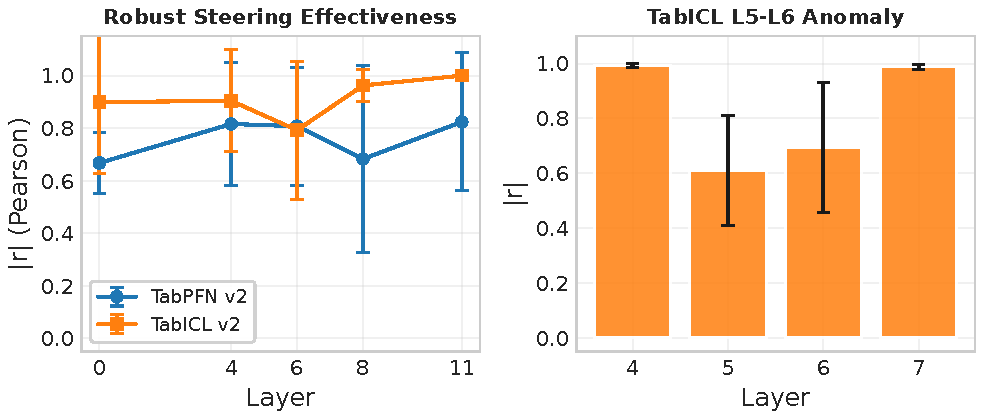
\includegraphics[width=0.75\textwidth]{figures/fig4_steering_and_anomaly.pdf}
  \caption{Steering effect profiles. Left: synthetic steering $|r|$ across layers for TabPFN and TabICL (10 seeds). Right: TabICL L6 anomaly --- highest variance, lowest steering strength among all layers.}
  \label{fig:app-steering}
\end{figure}

\begin{figure}[htbp]
  \centering
  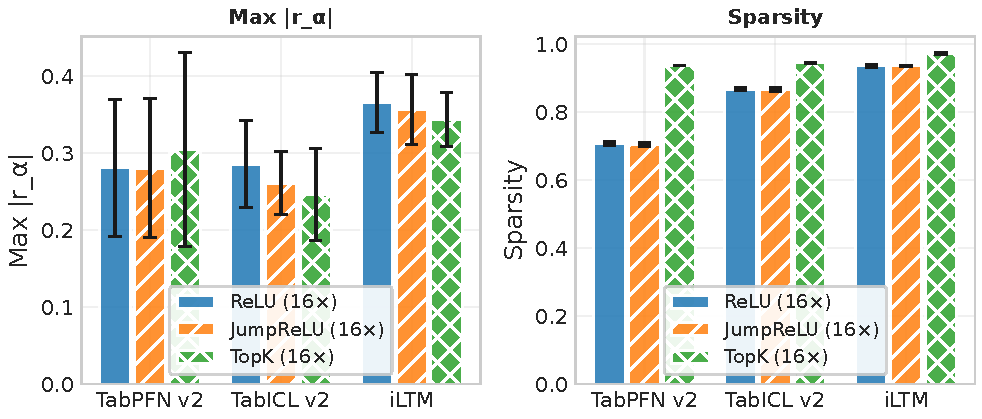
\includegraphics[width=0.75\textwidth]{figures/fig5_sae_comparison.pdf}
  \caption{SAE comparison: ReLU vs.\ TopK activation across models and layers. TopK achieves higher sparsity with comparable reconstruction, but monosemanticity ($|r_\alpha|$) remains low for both variants.}
  \label{fig:app-sae}
\end{figure}

\begin{figure}[htbp]
  \centering
  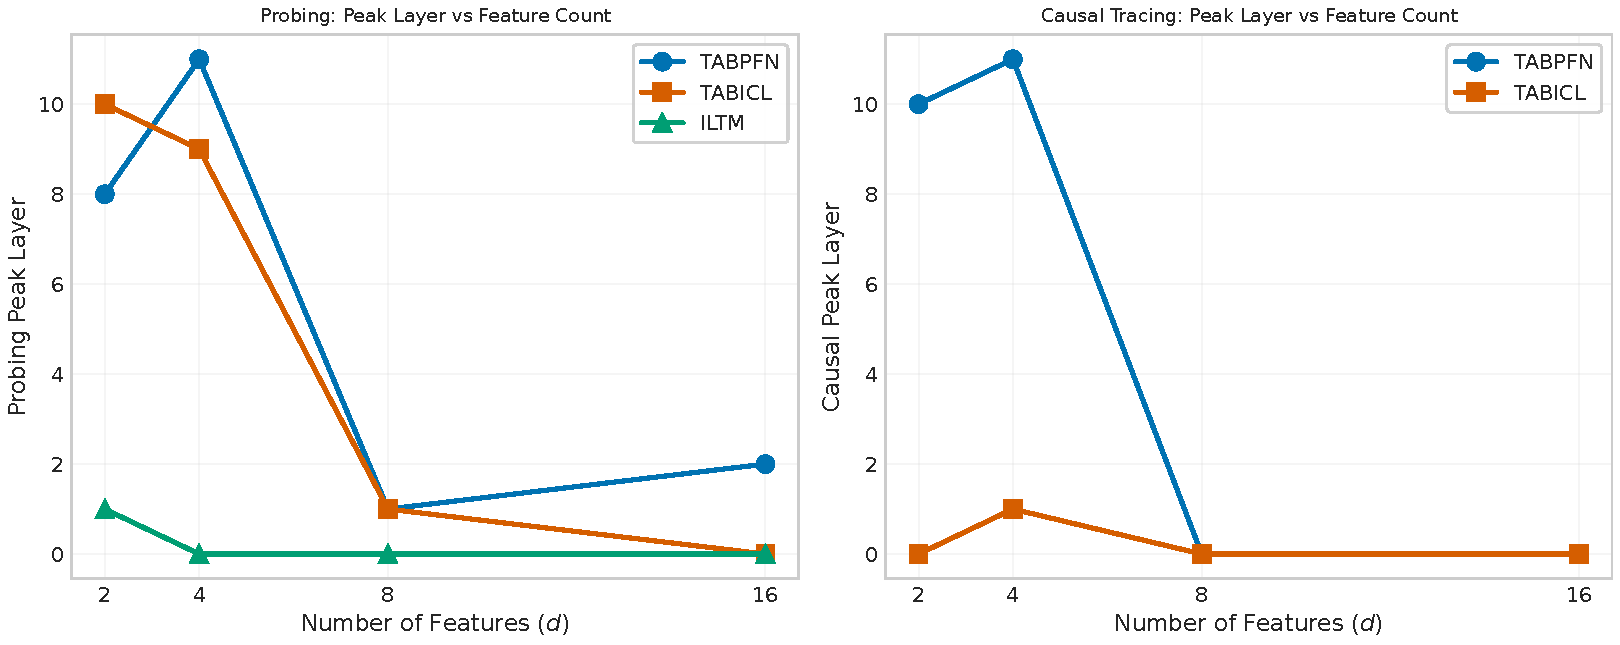
\includegraphics[width=\textwidth,height=4.5cm,keepaspectratio]{figures/fig9_feature_complexity.pdf}
  \caption{Feature complexity sweep ($d \in \{2, 4, 8, 16\}$): probing $R^2$ for the non-linear intermediary $\sin(x_0 \cdot x_1)$ as feature count increases. Probing degrades at $d \geq 8$ as the intermediary signal is drowned out by additional features; causal tracing remains informative.}
  \label{fig:app-feature-complexity}
\end{figure}

\begin{figure}[htbp]
  \centering
  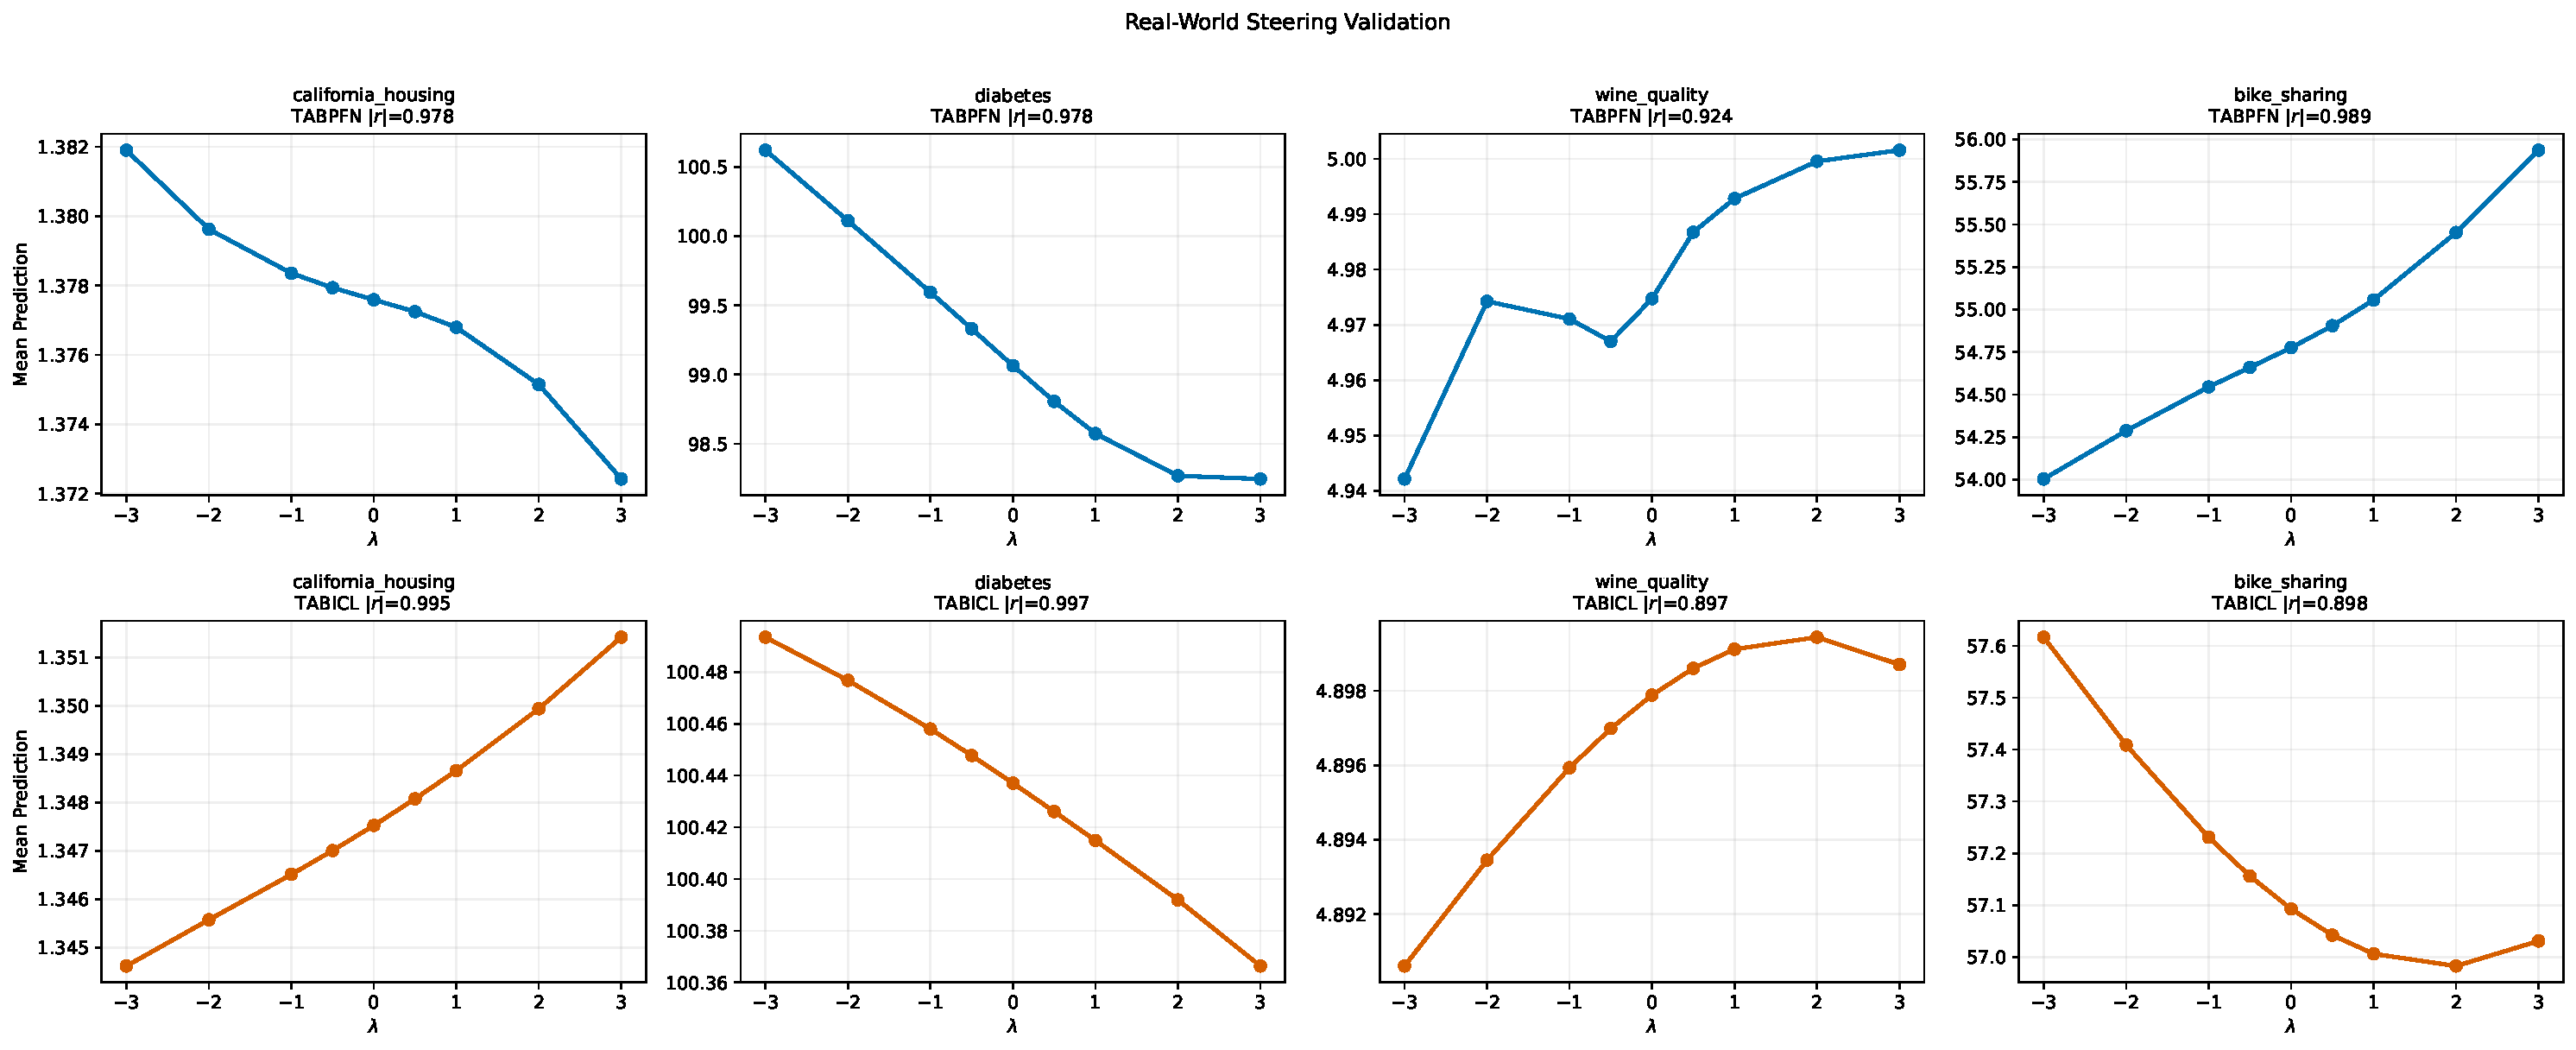
\includegraphics[width=\textwidth]{figures/fig10_realworld_steering.pdf}
  \caption{Real-world steering: prediction shift vs.\ steering strength ($\lambda$) on 4 regression datasets (seed 42). Both TabPFN (L6) and TabICL (L10) produce monotonic shifts ($|r| > 0.89$), providing proof-of-concept evidence that steering transfers beyond synthetic tasks.}
  \label{fig:app-realworld-steering}
\end{figure}

\section{Method Case Study: Full Table and Findings}
\label{app:method-case-study}

To demonstrate that TabMI-Bench is a usable evaluation tool rather than a one-off analysis, we applied the benchmark to three MI scoring methods: (M1)~\emph{linear probing} (Ridge, 5-fold cross-validated $R^2$); (M2)~\emph{activation-norm correlation} (per-sample $\|h\|_2$ vs.\ target); (M3)~\emph{variance-based importance} (average per-dim activation--target correlation). Each (method, model) pair was run over 5 seeds and assigned a label by the rule from \S3.

\begin{table}[htbp]
\centering
\caption{TabMI-Bench applicability labels generated by evaluating three MI methods on three core models (5 seeds, bilinear probe). Labels are derived from the \S3 rule, not hand-assigned. $^{*}$TabPFN cells marked \emph{Technical} due to dual-axis hook shape mismatch (150 vs.\ 50 tokens), a concrete gap documented in the release.}
\label{tab:method-case-study}
\small
\begin{tabular}{@{}l c c c@{}}
\toprule
Method & TabPFN & TabICL & iLTM \\
\midrule
Linear probing (M1) & Technical$^{*}$ & Supported & Supported \\
Activation-norm (M2) & Technical$^{*}$ & Supported & Limited \\
Variance-importance (M3) & Technical$^{*}$ & Supported & Supported \\
\bottomrule
\end{tabular}
\end{table}

\textbf{Findings.} On the 6 (TabICL, iLTM) cells where hook extraction succeeded, linear probing and variance-importance both receive \emph{Supported}, while activation-norm is \emph{Limited} on iLTM (tree preprocessing produces high-magnitude activations regardless of target, weakening norm-target correlation). The TabPFN \emph{Technical} outcome is itself a useful benchmark output: it surfaces a concrete uniformity gap in the hook interface for dual-axis TFMs, which the release addresses.

\section{Leave-One-Function-Out Robustness of the Primary Endpoint}
\label{app:lofo}

To verify that the primary-endpoint comparison ($\sigma^2_\text{profile}$ between TabPFN and TabICL) is not driven by any one synthetic function type, we repeat the comparison four times, each time holding out one of the four function types and using only the remaining three (across 5 seeds each). In every leave-one-out scenario the ordering $\sigma^2_\text{profile}(\text{TabPFN}) \gg \sigma^2_\text{profile}(\text{TabICL})$ is preserved with ratio $> 29\times$, and the minimum ratio is $29.6\times$ (hold out polynomial).

\begin{table}[htbp]
\centering
\caption{Leave-one-function-out robustness of the primary endpoint $\sigma^2_\text{profile}$ (intermediary probing, 5 seeds, 4 function types). For each held-out function the values are computed over the remaining 3 functions $\times$ 5 seeds ($n{=}15$). Source: \texttt{phase8a/nonlinear\_probing/lofo\_primary\_endpoint.json}.}
\label{tab:lofo}
\small
\begin{tabular}{@{}l c c c@{}}
\toprule
Held-out function & TabPFN $\sigma^2_\text{profile}$ & TabICL $\sigma^2_\text{profile}$ & Ratio \\
\midrule
Bilinear  & $0.083 \pm 0.022$ & $(2.1 \pm 2.5)\times10^{-3}$ & $39.0\times$ \\
Sinusoidal & $0.074 \pm 0.020$ & $(1.7 \pm 2.5)\times10^{-3}$ & $43.8\times$ \\
Polynomial & $0.094 \pm 0.016$ & $(3.2 \pm 2.4)\times10^{-3}$ & $29.6\times$ \\
Mixed      & $0.081 \pm 0.024$ & $(1.5 \pm 2.1)\times10^{-3}$ & $53.4\times$ \\
\midrule
All four (no holdout) & $0.083 \pm 0.022$ & $(2.1 \pm 2.5)\times10^{-3}$ & $39.0\times$ \\
\bottomrule
\end{tabular}
\end{table}

\noindent The staged-vs-distributed separation in the primary endpoint is therefore robust to removing any single function type. Per-layer $R^2$ values are clipped to $[-0.1, 1.0]$ prior to computing variance, to prevent outlier complexity levels from dominating. This clipping does not affect the TabPFN/TabICL ordering.

\section{Artifact Manifest}
\label{app:manifest}

For reviewer traceability, Table~\ref{tab:artifact-manifest} maps every numbered table and figure in the paper to its source artifact file and the script that generates it. All paths are relative to the repository root.

\begin{table}[htbp]
\centering
\caption{Artifact manifest: main-paper tables and figures $\to$ source JSON artifacts $\to$ generation scripts.}
\label{tab:artifact-manifest}
\scriptsize
\setlength{\tabcolsep}{3pt}
\begin{tabular}{@{}p{2.8cm} p{5.5cm} p{4.0cm}@{}}
\toprule
Paper element & Source artifact & Script \\
\midrule
Table 1 (3 strategies) & \texttt{rd5\_fullscale/aggregated/aggregated\_results.json} & \texttt{aggregate\_results.py} \\
Table 2 (bench.\ output) & N/A (design table) & --- \\
Table 3 (RW steering) & \texttt{phase8b/realworld\_steering\_multiseed/} & \texttt{phase8b\_multiseed\_runner.py} \\
Table 4 (evidence tiers) & N/A (index table) & --- \\
Table 5 (stats) & \texttt{paper/statistical\_report.md} & \texttt{statistical\_analysis.py} \\
Table 6 (seed regimes) & \texttt{rd5\_fullscale/run\_metadata.json} & --- \\
Table 7 (v2 vs v2.5) & \texttt{m28\_tabpfn25/results.json} & \texttt{rd6\_tabpfn25\_comparison.py} \\
Table 8 (applicability) & Multiple; see col.\ notes & --- \\
Table 9 (compute) & \texttt{*/run\_metadata.json} & --- \\
Table 10 (scaling) & \texttt{scale\_10k\_multiseed/results.json} & \texttt{run\_scale\_10k\_multiseed.py} \\
Fig 1 (intermediary) & \texttt{rd5\_fullscale/agg/*.json} + phase7 TabDPT & \texttt{generate\_paper\_figures.py} \\
Fig 2 (CKA heatmaps) & \texttt{rd5\_fullscale/seed\_*/cka/*.json} & \texttt{generate\_paper\_figures.py} \\
Fig 3 (causal + v2.5) & \texttt{rd5\_fullscale/*/patching/*.json}, \texttt{m28/*} & \texttt{generate\_paper\_figures.py} \\
Fig 7 (patch.\ vs noising) & \texttt{rd5\_fullscale/seed\_*/patching/*.json} & \texttt{generate\_paper\_figures.py} \\
Fig 8 (func.\ invariance) & \texttt{phase8a\_nonlinear\_probing/*seed*.json} & \texttt{generate\_phase8\_figures.py} \\
Fig seed-instability & \texttt{rd5\_fullscale/seed\_*/patching/*.json} & \texttt{generate\_seed\_instability\_figure.py} \\
\bottomrule
\end{tabular}
\end{table}

\textbf{Failed/retired runs disclosure.} The \texttt{rd6\_fullscale} canonical metadata records that two follow-up seed sweeps (seeds 789, 1024) hit a 7200s timeout on robust\_steering/improved\_sae/realworld\_expanded; the aggregated canonical file instead uses seeds \{42, 123, 456\} for which all experiments completed successfully. This policy is recorded in \texttt{rd6\_fullscale/run\_metadata.json} provenance annotation and in the aggregation script (filesystem-glob discovery over successful seed directories).

\textbf{Reproduce command.} From a clean clone with the environment set up via \texttt{requirements.txt}: \texttt{make reproduce-paper} runs aggregation, statistical analysis, and figure regeneration from frozen JSON artifacts (no GPU required at the reproduction stage; GPUs are only required for full re-runs from scratch).

\newpage
\section*{NeurIPS Paper Checklist}

\begin{enumerate}

\item {\bf Claims}
    \item[] Question: Do the main claims made in the abstract and introduction accurately reflect the paper's contributions and scope?
    \item[] Answer: \answerYes{}
    \item[] Justification: Abstract and \S1 claim (i)~a reusable hook-based MI infrastructure for 5 TFMs, (ii)~an evidence-coded applicability matrix with deterministic-cascading negative result, (iii)~three descriptive reference profiles as calibration. Each claim is backed by experimental evidence with explicit evidence tiers (Table~\ref{tab:evidence-tiers}) and seed-count annotations throughout.

\item {\bf Limitations}
    \item[] Question: Does the paper discuss the limitations of the work performed by the authors?
    \item[] Answer: \answerYes{}
    \item[] Justification: \S5.1 explicitly lists four categories of limitations: (i)~synthetic-probe/scale caveats, (ii)~design caveats including post-hoc taxonomy, iLTM 3-layer descriptive statistic, SAE moderate monosemanticity, steering $|r|$ saturation, (iii)~seed regimes per claim, (iv)~protocol-not-leaderboard scope. TabPFN causal-peak argmax instability is disclosed (Appendix~\ref{app:perseed}).

\item {\bf Theory assumptions and proofs}
    \item[] Answer: \answerNA{}
    \item[] Justification: This is an empirical benchmark paper; no theoretical claims or proofs are presented. Statistical plan (\S3) uses standard permutation/Welch/Wilcoxon tests without novel theoretical contribution.

\item {\bf Experimental result reproducibility}
    \item[] Answer: \answerYes{}
    \item[] Justification: All fixed seeds $\{42, 123, 456, 789, 1024\}$ for core experiments, hyperparameters, probe architectures, synthetic probe function definitions, and preprocessing steps are specified in \S3 and Appendix~\ref{app:architecture}. Hook implementations and data generators are part of the release. The artifact manifest (Appendix~\ref{app:manifest}) maps every numbered table/figure to its source JSON and generation script. A \texttt{make reproduce-paper} target regenerates all tables/figures from frozen JSON artifacts without GPU.

\item {\bf Open access to data and code}
    \item[] Answer: \answerYes{}
    \item[] Justification: Code, hook infrastructure for 5 TFMs, synthetic probe generators, configs, evaluation scripts, frozen JSON artifacts, \texttt{BENCHMARK\_CARD.md}, Croissant metadata (core + Responsible AI fields), and a worked example \texttt{examples/add\_new\_model.py} will be released on GitHub and Zenodo (DOI-minted) under the MIT license. External datasets used are public (scikit-learn, OpenML). Instructions and exact commands are documented in \texttt{README.md} and the Makefile.

\item {\bf Experimental setting/details}
    \item[] Answer: \answerYes{}
    \item[] Justification: Data splits ($N_\text{train}{=}100$, $N_\text{test}{=}50$ for core; $N_\text{train}{=}10$K / $N_\text{test}{=}1$K for scaling), optimizer/probe choices (Ridge regression with 5-fold CV), SAE variants (ReLU/JumpReLU/TopK with expansion factors $4{\times}$--$256{\times}$), and statistical plan (exact permutation as primary, Welch $t$ and Wilcoxon as sensitivity, per-seed unit-of-analysis) are specified in \S3 with full detail in Appendix~\ref{app:architecture}.

\item {\bf Experiment statistical significance}
    \item[] Answer: \answerYes{}
    \item[] Justification: Primary endpoints use exact permutation tests on per-seed summary statistics (avoiding per-layer pseudo-replication); Cohen's $d$ and bootstrap 95\% CIs are reported as sensitivity checks. Table~\ref{tab:stats} lists all 5 tests with raw $p$, effect sizes, and the pre-registered Bonferroni threshold $\alpha_{\text{Bonf}}=0.01$ (family-wise $\alpha=0.05$). Multi-seed figures report mean$\pm$1\,std shaded bands; per-seed tables (Appendix~\ref{app:perseed}) expose seed-level variation for transparency.

\item {\bf Experiments compute resources}
    \item[] Answer: \answerYes{}
    \item[] Justification: Appendix~\ref{app:compute} (Table~\ref{tab:compute}) reports hardware (128-core CPU; A100 80GB; 4$\times$A100), time per seed, peak memory, and number of retried runs per experiment family. Total compute: $\sim$40 GPU-hours (A100 80GB) + $\sim$20 CPU-hours. Retried/timed-out runs for rd6 (seeds 789/1024) are disclosed in the Failed/retired-runs note in the artifact manifest.

\item {\bf Code of ethics}
    \item[] Answer: \answerYes{}
    \item[] Justification: The research conforms to the NeurIPS Code of Ethics. No human subjects, no personal data collection, no dual-use concerns beyond general-purpose interpretability tooling. All external datasets are public and used under their permissive licenses. Anonymization is preserved in the submission.

\item {\bf Broader impacts}
    \item[] Answer: \answerYes{}
    \item[] Justification: Discussed in \S5 and expanded under the checklist's impact section: (+)~standardized MI evaluation for TFMs deployed in high-stakes domains (credit scoring, medical diagnosis, insurance pricing) enables auditing and supports regulatory compliance; (+)~the applicability matrix reduces wasted researcher effort. ($-$)~Risks: (1)~benchmark outputs are diagnostic measurements, not fairness/safety certification; (2)~a ``staged'' label does not guarantee full mechanistic understanding and could create false confidence; (3)~steering controllability demonstrated here is not policy-aligned safety controllability; (4)~the benchmark should sit inside a broader evaluation pipeline, not as standalone deployment approval.

\item {\bf Safeguards}
    \item[] Answer: \answerNA{}
    \item[] Justification: TabMI-Bench releases diagnostic tooling (hooks, probes, protocols, reference baselines), not pre-trained language models or generative models. The released artifacts pose no identified dual-use or high-misuse risk. All datasets used are public and pre-existing; no scraped or unfiltered web content is redistributed. The benchmark card documents intended uses and scope.

\item {\bf Licenses for existing assets}
    \item[] Answer: \answerYes{}
    \item[] Justification: All external datasets (OpenML datasets: California Housing, Diabetes, Wine Quality, Bike Sharing, Abalone, Boston, Energy Efficiency, Breast Cancer, Iris, Adult Income, Credit-G, Concrete) and models (TabPFN v2/v2.5, TabICL v2, TabDPT, iLTM, NAM) are cited with their original publications and used under their permissive licenses (e.g., scikit-learn: BSD; OpenML: CC-BY; model checkpoints: as per original releases). Version strings and source URLs are documented in Appendix~\ref{app:architecture} and the benchmark card.

\item {\bf New assets}
    \item[] Answer: \answerYes{}
    \item[] Justification: TabMI-Bench (new asset) is released under the MIT license with: (a)~\texttt{BENCHMARK\_CARD.md} documenting intended uses, scope, failure modes, and provenance; (b)~Croissant metadata (\texttt{croissant.json}) covering both core and Responsible AI fields for the synthetic probes and hook infrastructure; (c)~a worked example (\texttt{examples/add\_new\_model.py}) and \texttt{HookedModel} interface documentation; (d)~frozen JSON artifacts for all main-paper tables/figures; (e)~per-seed result tables (Appendix~\ref{app:perseed}). At submission time, all assets are provided through anonymized URLs / zip file.

\item {\bf Crowdsourcing and research with human subjects}
    \item[] Answer: \answerNA{}
    \item[] Justification: No crowdsourcing, no human subjects, no human-labeled data collected for this work.

\item {\bf Institutional review board (IRB) approvals or equivalent for research with human subjects}
    \item[] Answer: \answerNA{}
    \item[] Justification: No human subjects research; IRB review is not applicable.

\item {\bf Declaration of LLM usage}
    \item[] Answer: \answerNA{}
    \item[] Justification: Anthropic's Claude and OpenAI's Codex assisted with (i)~English drafting and \LaTeX{} source editing/auditing, (ii)~academic-style polishing, and (iii)~Python code review and error fixes for author-identified bug patches. These tools did not design experiments, generate empirical results, choose baselines, or alter any reported number; all scientific decisions and final wording are the authors' responsibility. No LLM is therefore an original or non-standard component of the research.

\end{enumerate}

\end{document}
